\documentclass[9pt]{beamer}
\usepackage[utf8]{inputenc}
\usepackage[russian,english]{babel}
\usepackage{graphicx, epsfig}
\usepackage{amsmath,mathrsfs,amsfonts,amssymb}
\usepackage{subfig}
\usepackage{floatflt}
\usepackage{epic,ecltree}
\usepackage{mathtext}
\usepackage{fancybox}
\usepackage{fancyhdr}
\usepackage{multirow}
\usepackage{enumerate}
\usepackage{epstopdf}
\usepackage{multicol}
\usepackage{algorithm}
\usepackage[noend]{algorithmic}
\def\algorithmicrequire{\textbf{Input:}}
\def\algorithmicensure{\textbf{Output:}}
\usetheme{Singapore}%{Singapore}%{Warsaw}%{Warsaw}%{Darmstadt}
\usecolortheme{default}
\setbeamertemplate{footline}[page number]{}
\newcommand{\bx}{\mathbf{x}}
\newcommand{\by}{\mathbf{y}}
\newcommand{\bz}{\mathbf{z}}
\newcommand{\bw}{\mathbf{w}}
\newcommand{\ba}{\mathbf{a}}
\newcommand{\bb}{\mathbf{b}}
\newcommand{\bY}{\mathbf{Y}}
\newcommand{\bX}{\mathbf{X}}
\newcommand{\bu}{\mathbf{u}}
\newcommand{\bt}{\mathbf{t}}
\newcommand{\bp}{\mathbf{p}}
\newcommand{\bq}{\mathbf{q}}
\newcommand{\bc}{\mathbf{c}}
\newcommand{\bP}{\mathbf{P}}
\newcommand{\bT}{\mathbf{T}}
\newcommand{\bB}{\mathbf{B}}
\newcommand{\bQ}{\mathbf{Q}}
\newcommand{\bC}{\mathbf{C}}
\newcommand{\bE}{\mathbf{E}}
\newcommand{\bF}{\mathbf{F}}
\newcommand{\bU}{\mathbf{U}}
\newcommand{\bW}{\mathbf{W}}
\newcommand{\bbR}{\mathbb{R}}
\newcommand{\cA}{\mathcal{A}}
\newcommand{\bchi}{\boldsymbol{\chi}}
\newcommand{\bnu}{\boldsymbol{\nu}}
\newcommand{\bmu}{\boldsymbol{\mu}}
\newcommand{\bOne}{\boldsymbol{1}}
\newcommand{\bZero}{\boldsymbol{0}}
\newcommand{\btheta}{\boldsymbol{\theta}}
\newcommand{\bTheta}{\boldsymbol{\Theta}}
\newcommand{\argmin}{\mathop{\arg \min}\limits}
\newcommand{\argmax}{\mathop{\arg \max}\limits}

\newcommand\undermat[2]{%
	\makebox[0pt][l]{$\smash{\underbrace{\phantom{%
					\begin{matrix}#2\end{matrix}}}_{\text{$#1$}}}$}#2}

\newtheorem{statement}{Statement}

\usepackage{tikz-cd}
%\definecolor{beamer@blendedblue}{RGB}{15,120,80}
%----------------------------------------------------------------------------------------------------------
\title[\hbox to 56mm{  \hfill\insertframenumber\,/\,\inserttotalframenumber}]
{\\ \vspace{1.5cm} Signal Decoding in multicorrelated high-dimensional spaces}
\author[Roman Isachenko]{\\ 
	\vspace{.4cm}
	Roman Isachenko}
\institute[SkolTech]{Skoltech advisor: Maxim Fedorov \\ 
	\vspace{0.1cm}
	 MIPT advisor: Vadim Strijov
}
\date{April 27, 2018.}
%--------------------------------------------------------------------------------
\begin{document}
%--------------------------------------------------------------------------------
\begin{frame}
%\thispagestyle{empty}
\titlepage
\end{frame}
%--------------------------------------------------------------------------------
\begin{frame}{Signal decoding problem}
	\begin{block}{Goal}
		\begin{itemize}
			\item Investigate input, latent, and target spaces for signal decoding problem.
			\item Build a stable model for time series decoding in the case of multicorrelated object description.
			\item Suggest dimensionality reduction algorithm for signal decoding problem.
		\end{itemize}
	\end{block}
	\begin{block}{Challenge}
		\begin{itemize}
			\item Measurements of spatial-temporal data are interacted since sensors are close to each other.
			\item Target variable is a vector whose elements are dependent.
		\end{itemize}
	\end{block}
	\begin{block}{Solution}
		Propose to use joint description of independent and target variables. This description allows to reduce the multicorrelation and to build stable adequate model with acceptable accuracy.
	\end{block}
\end{frame}
%--------------------------------------------------------------------------------
\begin{frame}{Related works}
	\begin{itemize}
		\item Katrutsa A., Strijov V. Comprehensive study of feature selection methods to solve multicollinearity problem according to evaluation criteria. // \textit{Expert Systems with Applications} 76, 2017.
		\vfill
		\item Li J. et al. Feature selection: A data perspective //\textit{ACM Computing Surveys (CSUR)} 50(6), 2017.
		\vfill
		\item Eliseyev A. et al. Iterative N-way partial least squares for a binary self-paced brain–computer interface in freely moving animals //\textit{Journal of neural engineering} 4(8), 2011.
		\vfill
		\item Rodriguez-Lujan I. et al. Quadratic programming feature selection // \textit{Journal of Machine Learning Research} 11(Apr), 2010.
		\vfill
		\item Motrenko A., Strijov V. Multi-way Feature Selection for ECoG-based Brain-Computer Interface // \textit{Expert Systems with Applications} Submitted to the journal.
	\end{itemize}
\end{frame}
%--------------------------------------------------------------------------------
\begin{frame}{Application: Brain Computer Interface (BCI)}
	\begin{minipage}{0.58\linewidth}
		\begin{block}{Aim}
		Develop systems to help people with a severe motor control disability recover mobility.
		\end{block}
	\begin{block}{Hypothesis}
	"When we imagine making a movement, we trigger the same electrical activity in the motor cortex of the brain as when we actually perform that activity."$^*$
	\end{block}
	\begin{block}{Solution}
	Record electrical signals~-- electrocorticograms (ECoG), decode them to drive complex objects, for example, to move the limbs of an exoskeleton. 
	\end{block}
	$^*$ \url{http://clinatec.fr};
	\end{minipage}%
\begin{minipage}{0.4\linewidth}
	\centering
	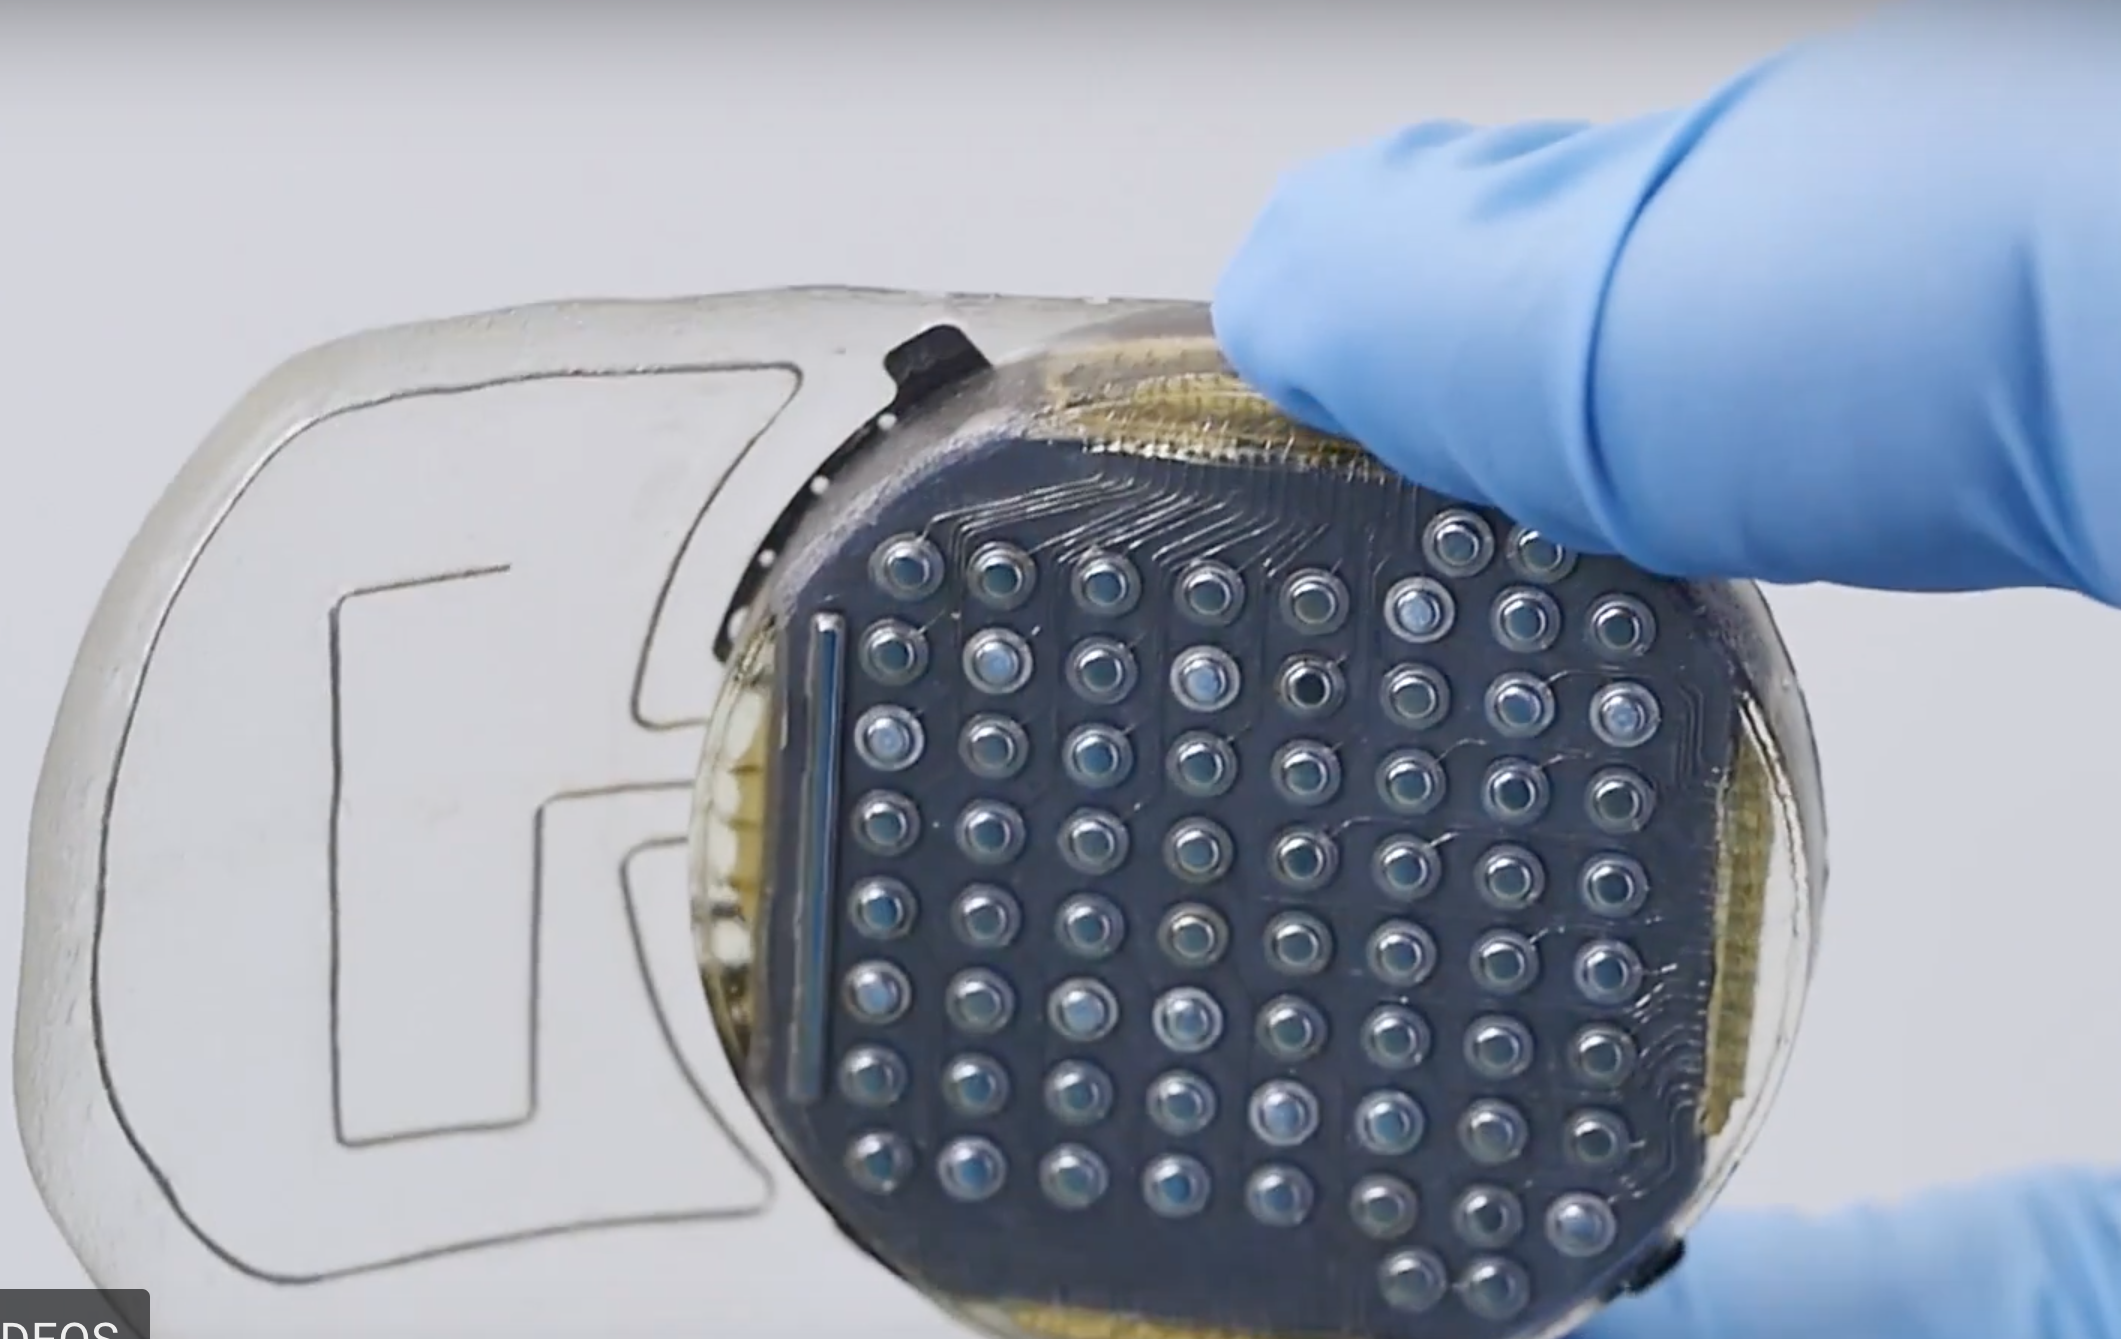
\includegraphics[width=0.9\linewidth]{figs/deviceClinatec} \\
	\vspace{0.5cm}
	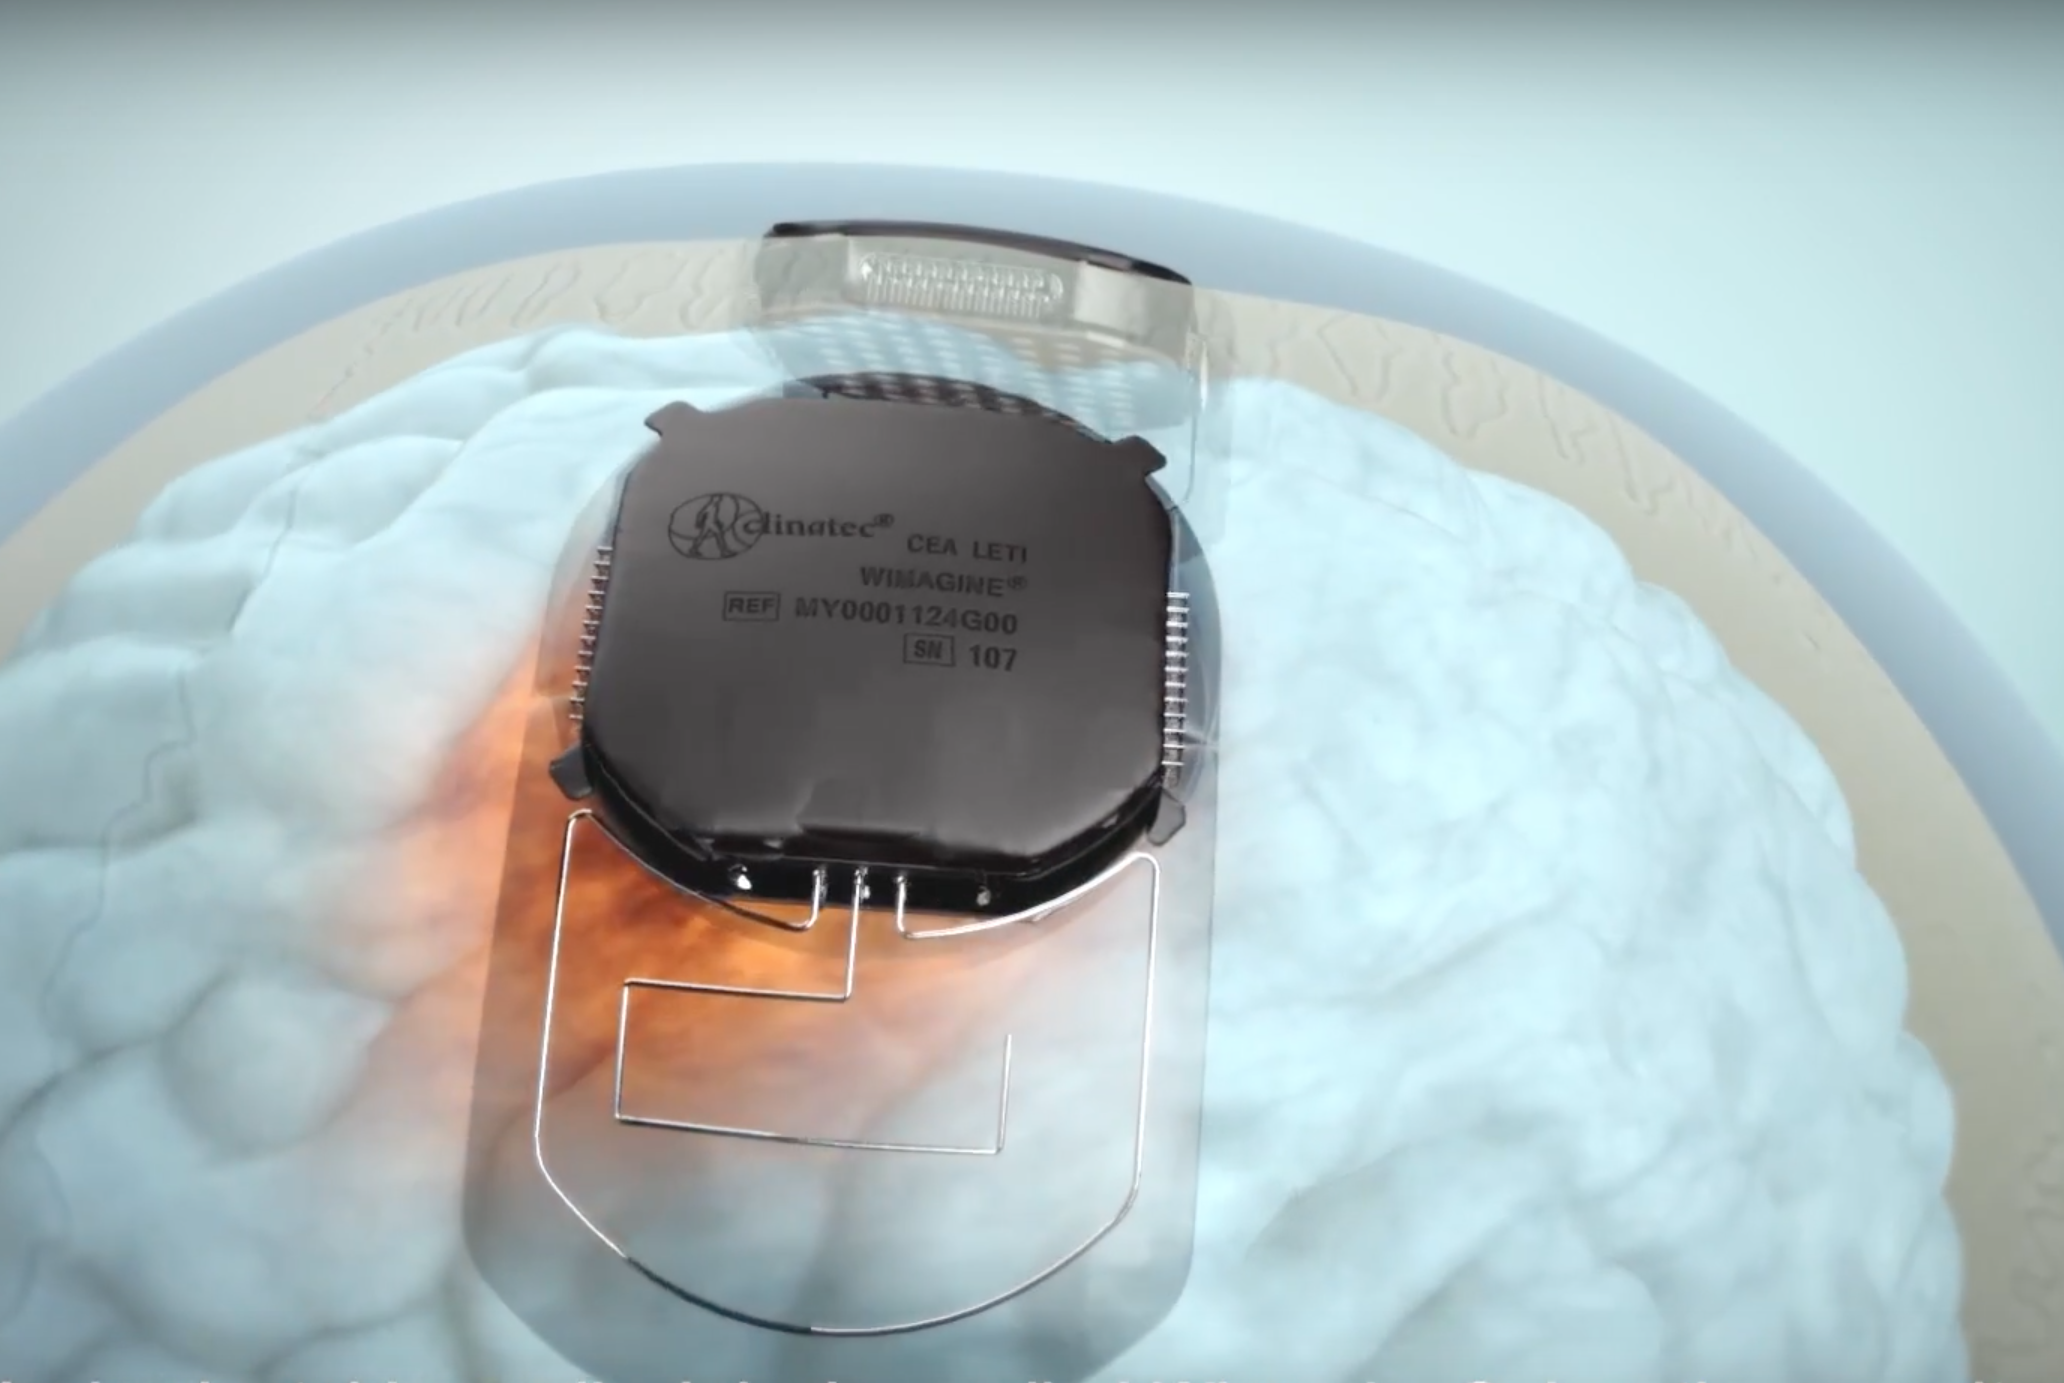
\includegraphics[width=0.9\linewidth]{figs/brainClinatec}
\end{minipage}
\vspace{0.3cm} \\
\hrulefill \\
\small{Eliseyev A. et al. CLINATEC BCI platform based on the ECoG-recording implant WIMAGINE and the innovative signal-processing: preclinical results, 2014.}
\end{frame}
%--------------------------------------------------------------------------------
\begin{frame}{Multivariate regression}
	\begin{block}{Model}
	Forecast a dependent variable $\by \in \bbR^r$ from an independent input object $\bx \in \bbR^n$
	\[
	\by = \bTheta \bx+ \boldsymbol{\varepsilon}, \quad \bTheta \in \bbR^{r \times n}
	\]
	\vspace{-0.7cm}
	\end{block}
	\begin{block}{Given}
	Dataset $\left( \bX, \bY \right)$, design matrix~$\bX \in \bbR^{m \times n}$, target matrix~$\bY \in \bbR^{m \times r}$,
	\[
	\bX = [\bx_1, \dots, \bx_m]^{T} =  [\bchi_1, \dots, \bchi_n]; \quad \bY = [\by_1, \dots, \by_m]^{T} =  [\bnu_1, \dots, \bnu_r].
	\]
	\vspace{-0.7cm}
	\end{block}
	\begin{block}{Error function}
	\[
	S(\bTheta | \bX, \bY) = {\left\| \underset{m \times r}{\mathbf{Y}}  - \underset{m \times n}{\bX} \cdot \underset{r \times n}{\bTheta}^T \right\| }_2^2 \rightarrow\min_{\bTheta}.
	\label{eq:error_function}
	\]
	\[
	\bTheta = (\bX^{T} \bX)^{-1} \bX^{T} \bY.
	\]
	\end{block}
	The linear dependent columns of the matrix $\bX$ leads to an instable solution. \\
	To avoid the strong linear dependence, feature selection and dimensionality reduction techniques are used.
\end{frame}

%--------------------------------------------------------------------------------
\begin{frame}{Feature selection problem statement}
\begin{block}{Goal}
Find the index set~$\cA = \{1, \dots, n\}$ of~$\bX$ columns. 
\end{block}
\begin{block}{Quality Criteria}
To select the set~$\cA$ among all possible $2^n - 1$ subsets, introduce the feature selection quality criteria
\[
\cA = \argmax_{\cA' \subseteq \{1, \dots, n\}} Q(\cA' | \bX, \bY).
\label{eq:subset_selection}
\]
\end{block}
Once the solution~$\cA$ is known:
\[
S(\bTheta_{\cA} | \bX_{\cA}, \bY) = {\left\| \mathbf{Y} - \bX_{\cA}\bTheta^T_{\cA} \right\| }_2^2 \rightarrow\min_{\bTheta_{\cA}},
\]
where the subscript~$\cA$ indicates columns with indices from the set~$\cA$.

\end{frame}
%--------------------------------------------------------------------------------
\begin{frame}{Quadratic Programming Feature Selection}
	\[
	\| \bnu - \bX \btheta\|_2^2 \rightarrow\min_{\btheta \in \bbR^{n}}.
	\]
	\begin{block}{Quadratic Programming Feature Selection}
	\vspace{-0.3cm}
	\[
	(1 - \alpha) \cdot \underbrace{\ba^{T} \bQ \ba}_{\text{Sim}(\bX)} - \alpha \cdot \underbrace{\vphantom{()} \mathbf{b}^{T} \ba}_{\text{Rel}(\bX, \bnu)} \rightarrow \min_{\substack{\ba \geq \bZero_n \\ \bOne_n^T \ba=1}}.
	\]
	\vspace{-0.3cm}
	\end{block}
		\begin{itemize}
			\item $\ba \in \bbR^n$ --- feature importances;
			\item $\bQ \in \bbR^{n \times n}$ - pairwise feature similarities;
			\item $\mathbf{b} \in \bbR^n$ - feature relevances to the target vector.
		\end{itemize}
	
	\begin{equation*}
	j \in \mathcal{A}^* \Leftrightarrow a_j > \tau
	\end{equation*}
	
	\begin{block}{Quality Criteria}
	\[
	\cA = \argmax_{\cA' \subseteq \{1, \dots, n\}} Q(\cA' | \bX, \bnu) \Leftrightarrow \argmin_{\ba \geq \bZero_n, \, \bOne_n^T\ba=1} \bigl[\ba^{T} \bQ \ba - \alpha \cdot \mathbf{b}^{T} \ba \bigr].
	\]
	\end{block}
\end{frame}
%--------------------------------------------------------------------------------
\begin{frame}{Quadratic Programming Feature Selection}
	
	\begin{block}{Quality Criteria}
		\[
		\cA = \argmax_{\cA' \subseteq \{1, \dots, n\}} Q(\cA' | \bX, \bnu) \Leftrightarrow \argmin_{\ba \geq \bZero_n, \, \bOne_n^T\ba=1} \bigl[\ba^{T} \bQ \ba - \alpha \cdot \mathbf{b}^{T} \ba \bigr].
		\]
		\vspace{-0.5cm}
	\end{block}
	\begin{block}{Similarity measure}
		\begin{itemize}
			\item Correlation
			\vspace{-0.1cm}
			\[
			\left|\text{corr}(\bx, \by)\right| = \left| \frac{\mathrm{cov}(\bx, \by)}{\sqrt{\mathrm{Var}(\bx) \mathrm{Var}(\by)}} \right|
			\]
			\vspace{-0.3cm}
			\item Mutual information
			\vspace{-0.1cm}
			\[
			I(\bx, \by) = \int \int p(\bx, \by) \log \frac{p(\bx, \by)}{p(\bx) p(\by)} d\bx d\by.
			\]
			\vspace{-0.5cm}
		\end{itemize}
	\end{block}
	\[
	\bQ = \left\{\left|\text{corr}(\bchi_i, \bchi_j)\right|\right\}_{i,j=1}^n, \quad \bb = \left\{\left|\text{corr}(\bchi_i, \bnu)\right|\right\}_{i=1}^n.
	\]
	\vspace{-0.5cm}
	\begin{block}{Statement}
		In the case of semidefinite matrix $\bQ$ the QPFS problem is convex.
	\end{block}
	\begin{equation*}
	\bQ \rightarrow \bQ - \lambda_{\min} \mathbf{I}	
	\end{equation*}
\end{frame}
%--------------------------------------------------------------------------------
\begin{frame}{Multivariate QPFS}
\begin{block}{Relevance aggregation}
\vspace{-0.3cm}
\[
\bQ = \left\{\left|\text{corr}(\bchi_i, \bchi_j)\right|\right\}_{i,j=1}^n, \quad \bb = \left\{\sum_{k=1}^r\left|\text{corr}(\bchi_i, \bnu_k)\right|\right\}_{i=1}^n.
\]
\vspace{-0.3cm}
\end{block}

This approach does not use the dependencies in the columns of the matrix $\bY$. 
	
\begin{block}{Example:}
\vspace{-0.5cm}
\[
\bX = [\bchi_1, \bchi_2, \bchi_3], \quad \bY = [\underbrace{\bnu_1, \bnu_1, \dots, \bnu_1}_{r-1}, \bnu_2],
\]
\vspace{-0.2cm}
\[
\bQ = \begin{bmatrix} 1 & 0 & 0\\ 0 & 1 & 0.8 \\ 0 & 0.8 & 1 \end{bmatrix}, \quad 
\bB = \begin{bmatrix} 0.4 & \dots & 0.4 & 0 \\ 0.5 & \dots & 0.5 & 0.8 \\ \undermat{r-1}{0.8 & \dots & 0.8} & 0.1 \end{bmatrix}, \quad
\bb = \begin{bmatrix} (r-1) \cdot 0.4 + 0 \\ (r-1) \cdot 0.5 + 0.8 \\ (r-1) \cdot 0.8 + 0.1 \end{bmatrix}
\]
\end{block}
\vspace{0.2cm}

Best subset: $[\bchi_1, \bchi_2]$. \\
\vspace{0.2cm}
QPFS ($r=2$): $\ba = [\mathbf{0.37},	\mathbf{0.61},	0.02]$. \\
QPFS ($r=5$): ~$\ba = [\mathbf{0.40},	0.17, \mathbf{0.43}]$. 
\end{frame}
%--------------------------------------------------------------------------------
\begin{frame}{Symmetric Importance}
Penalize correlated targets by $\text{Sim} (\bY)$
\[
\alpha_1 \cdot \underbrace{\ba_x^{T} \bQ_x \ba_x}_{\text{Sim}(\bX)} - \alpha_2 \cdot \underbrace{\ba_x^{T} \bB \ba_y}_{\text{Rel}(\bX, \bY)} + \alpha_3 \cdot \underbrace{\ba_y^{T} \bQ_y \ba_y}_{\text{Sim}(\bY)} \rightarrow \min_{\substack{\ba_x \geq \bZero_n, \, \bOne_n^T\ba_x=1 \\ \ba_y \geq \bZero_r, \, \bOne_r^T\ba_y=1}}.
\]
\[
\bQ_x = \left\{ \left| \text{corr}(\bchi_i, \bchi_j) \right| \right\}_{i,j=1}^n, \,
\bQ_y = \left\{ \left| \text{corr}(\bnu_i, \bnu_j) \right| \right\}_{i,j=1}^r, \,
\bB =  \left\{ \left| \text{corr}(\bchi_i, \bnu_j) \right| \right\}_{\substack{i=1, \dots, n \\ j=1, \dots, r}}.
\]
\[
\alpha_1 + \alpha_2 + \alpha_3 = 1 \quad \alpha_i \geq 0, \, i = 1, 2, 3.
\] 

\begin{statement}
	Balance between the terms $\text{Sim}(\bX)$ and $\text{Rel}(\bX, \bY)$ for the problem is achieved by the following coefficients:
	\vspace{-0.2cm}
	\[
	\alpha_1 = \frac{(1 - \alpha_3)\overline{\bB}}{\overline{\bQ}_x + \overline{\bB}}; \quad
	\alpha_2 = \frac{(1 - \alpha_3)\overline{\bQ}_x}{\overline{\bQ}_x + \overline{\bB}}; \quad
	\alpha_3 \in [0, 1],
	\]
	where $\overline{\bQ}_x$, $\overline{\bB}$ are the mean values of~$\bQ_x$ and $\bB$ respectively.
\end{statement}
\end{frame}
%--------------------------------------------------------------------------------
\begin{frame}{Multivariate QPFS}
	\begin{block}{Example:}
		\vspace{-0.5cm}
		\[
		\bX = [\bchi_1, \bchi_2, \bchi_3], \quad \bY = [\underbrace{\bnu_1, \bnu_1, \dots, \bnu_1}_{r-1}, \bnu_2],
		\]
		\vspace{-0.2cm}
		\[
		\bQ = \begin{bmatrix} 1 & 0 & 0\\ 0 & 1 & 0.8 \\ 0 & 0.8 & 1 \end{bmatrix}, \quad 
		\bB = \begin{bmatrix} 0.4 & \dots & 0.4 & 0 \\ 0.5 & \dots & 0.5 & 0.8 \\ \undermat{r-1}{0.8 & \dots & 0.8} & 0.1 \end{bmatrix}, \quad
		\bb = \begin{bmatrix} (r-1) \cdot 0.4 + 0 \\ (r-1) \cdot 0.5 + 0.8 \\ (r-1) \cdot 0.8 + 0.1 \end{bmatrix}
		\]
	\end{block}
	\vspace{0.2cm}
	\begin{center}
$\bQ_x = \bQ$; $\bQ_y:$ $\text{corr}(\bnu_1, \bnu_2) = 0.2$ all others entries = 1. 
\end{center}
Best subset: $[\bchi_1, \bchi_2]$.
\begin{figure}
	\centering
	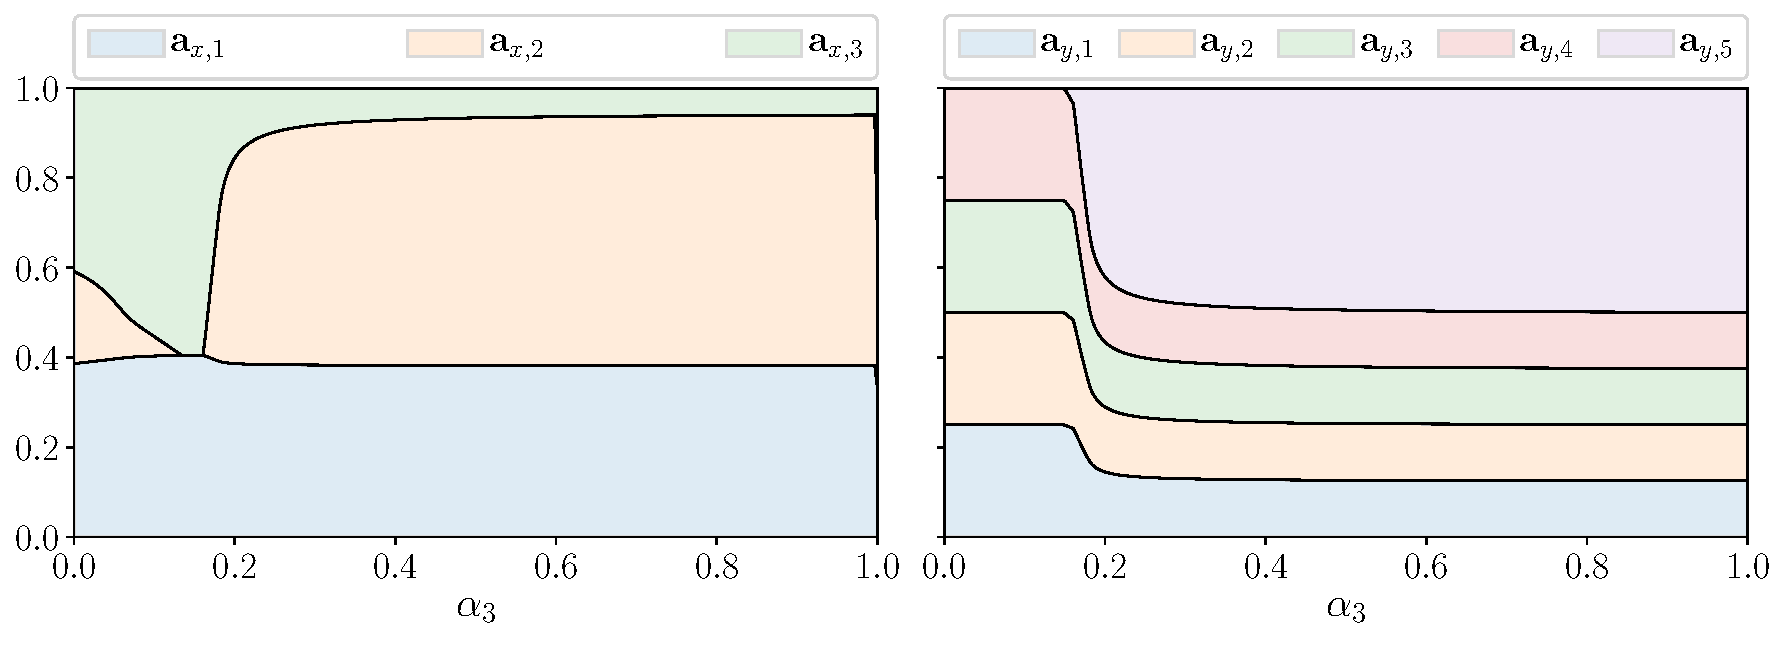
\includegraphics[width=\linewidth]{figs/features_vs_alpha.pdf}
\end{figure}
\end{frame}
%--------------------------------------------------------------------------------
\begin{frame}{Min-max / Max-min}
	Symmetric Importances penalizes targets that are correlated and are not sufficiently explained by the features. 
	\[
	\alpha_1 \cdot \underbrace{\ba_x^T \bQ_x \ba_x}_{\text{Sim}(\bX)} - \alpha_2 \cdot \underbrace{\vphantom{()} \ba_x^T\mathbf{B} \ba_y}_{\text{Rel}(\bX, \bY)} \rightarrow \min_{\substack{\ba_x \geq \bZero_n, \\ \bOne_n^T\ba_x=1}}; \quad
	\alpha_3 \cdot \underbrace{\ba_y^T \bQ_y \ba_y}_{\text{Sim}(\bY)} + \alpha_2 \cdot \underbrace{\vphantom{()} \ba_x^T \mathbf{B} \ba_y}_{\text{Rel}(\bX, \bY)} \rightarrow \min_{\substack{\ba_y \geq \bZero_r,  \\ \bOne_r^T\ba_y=1}}.
	\]
	\begin{block}{Min-max / Max-min}
	\vspace{-0.5cm}
	\[
	\min_{\substack{\ba_x \geq \bZero_n \\ \bOne_n^T\ba_x=1}} 	\max_{\substack{\ba_y \geq \bZero_r \\ \bOne_r^T\ba_y=1}} \left(\text {or} \, \max_{\substack{\ba_y \geq \bZero_r \\ \bOne_r^T\ba_y=1}} \min_{\substack{\ba_x \geq \bZero_n \\ \bOne_n^T\ba_x=1}}\right) \left[\alpha_1 \cdot \underbrace{\ba_x^T \bQ_x \ba_x}_{\text{Sim}(\bX)} - \alpha_2 \cdot \underbrace{\ba_x^T \bB \ba_y}_{\text{Rel}(\bX, \bY)} - \alpha_3 \cdot \underbrace{\ba_y^T \bQ_y \ba_y}_{\text{Sim}(\bY)}\right].
	\]
	\end{block}
	\[
	\cA = \argmax_{\cA' \subseteq \{1, \dots, n\}} Q(\cA' | \bX, \bY) \Leftrightarrow \argmin_{\ba_x \geq \bZero_n, \, \bOne_n^T\ba_x=1} \left[\max_{\substack{\ba_y \geq \bZero_r \\ \bOne_r^T\ba_y=1}} f(\ba_x, \ba_y)\right].
	\]
	\begin{theorem}
		For positive definite matrices $\bQ_x$ and $\bQ_y$ the max-min and min-max problems have the same optimal value. 
	\end{theorem}

\end{frame}
%--------------------------------------------------------------------------------
\begin{frame}{Min-max / Max-min}
	
	\begin{block}{Lagrangian for fixed~$\ba_x$}
	\vspace{-0.4cm}
	\[
	L(\ba_x, \ba_y, \lambda, \bmu) = \alpha_1 \cdot \ba_x^T \bQ_x \ba_x - \alpha_2 \cdot \ba_x^T \bB \ba_y - \alpha_3 \cdot \ba_y^T \bQ_y \ba_y + \lambda \cdot  (\bOne_r^T \ba_y - 1) + \bmu^T \ba_y.
	\]
	\end{block}
	\vspace{-0.2cm}
	\begin{block}{Theorem}
	Min-max problem is equivalent to the following quadratic problem with $n + r + 1$ variables
	\[
	\min_{\substack{\ba_x \geq \bZero_n, \, \bOne_n^T\ba_x=1 \\ \lambda, \, \bmu \geq \bZero_r}} g(\ba_y, \lambda, \bmu), \quad \text{where}
	\]
	\end{block}
	\vspace{-.8cm}
	\begin{multline*}
	g(\ba_x, \lambda, \bmu) 
	= \max_{\ba_y \in \bbR^r} L(\ba_x, \ba_y, \lambda, \bmu) = 
	\ba_x^T \left( - \frac{\alpha_2^2}{4\alpha_3} \bB \bQ_y^{-1} \bB^T - \alpha_1 \cdot \bQ_x\right) \ba_x \\ - \frac{1}{4 \alpha_3} \lambda^2 \cdot \bOne_r^T \bQ_y^{-1} \bOne_r - \frac{1}{4 \alpha_3} \bmu^T \bQ_y^{-1} \bmu + \frac{\alpha_2}{2 \alpha_3} \lambda \cdot \bOne_r^T \bQ_y^{-1} \bB^T \ba_x \\ - \frac{1}{2 \alpha_3} \lambda \cdot \bOne_r^T \bQ_y^{-1} \bmu + \frac{\alpha_2}{2 \alpha_3} \bmu^T \bQ_y^{-1} \bB^T \ba_x + \lambda. 
	\end{multline*} 
	The problem is not convex. If we shift the spectrum for the matrix of quadratic form, the optimality is lost. 
\end{frame}
%--------------------------------------------------------------------------------
\begin{frame}{Minimax Relevances}
	Drop the term~$\text{Sim}(\bY)$. 
	\[
		\min_{\substack{\ba_x \geq \bZero_n \\ \bOne_n^T\ba_x=1}} 	\max_{\substack{\ba_y \geq \bZero_r \\ \bOne_r^T\ba_y=1}} \left[ (1 - \alpha) \cdot \ba_x^T \bQ_x \ba_x - \alpha \cdot \ba_x^T \bB \ba_y \right].
	\]
	\begin{block}{Dual function}
	\[
	g(\ba_x, \lambda, \bmu) =
	\begin{cases}
	(1 - \alpha) \cdot \ba_x^T \bQ_x \ba_x - \lambda, & \alpha \cdot \bB^T \ba_x = \lambda \cdot \bOne_r + \bmu;  \\
	+ \infty, & \text{otherwise}.
	\end{cases}
	\]
	\end{block}
\begin{statement}
	For the case $r=1$ the proposed strategies coincide with the original QPFS algorithm.
\end{statement}
	
\end{frame}
%--------------------------------------------------------------------------------
\begin{frame}{Computational experiment}
\begin{block}{Data example}
	\begin{figure}
		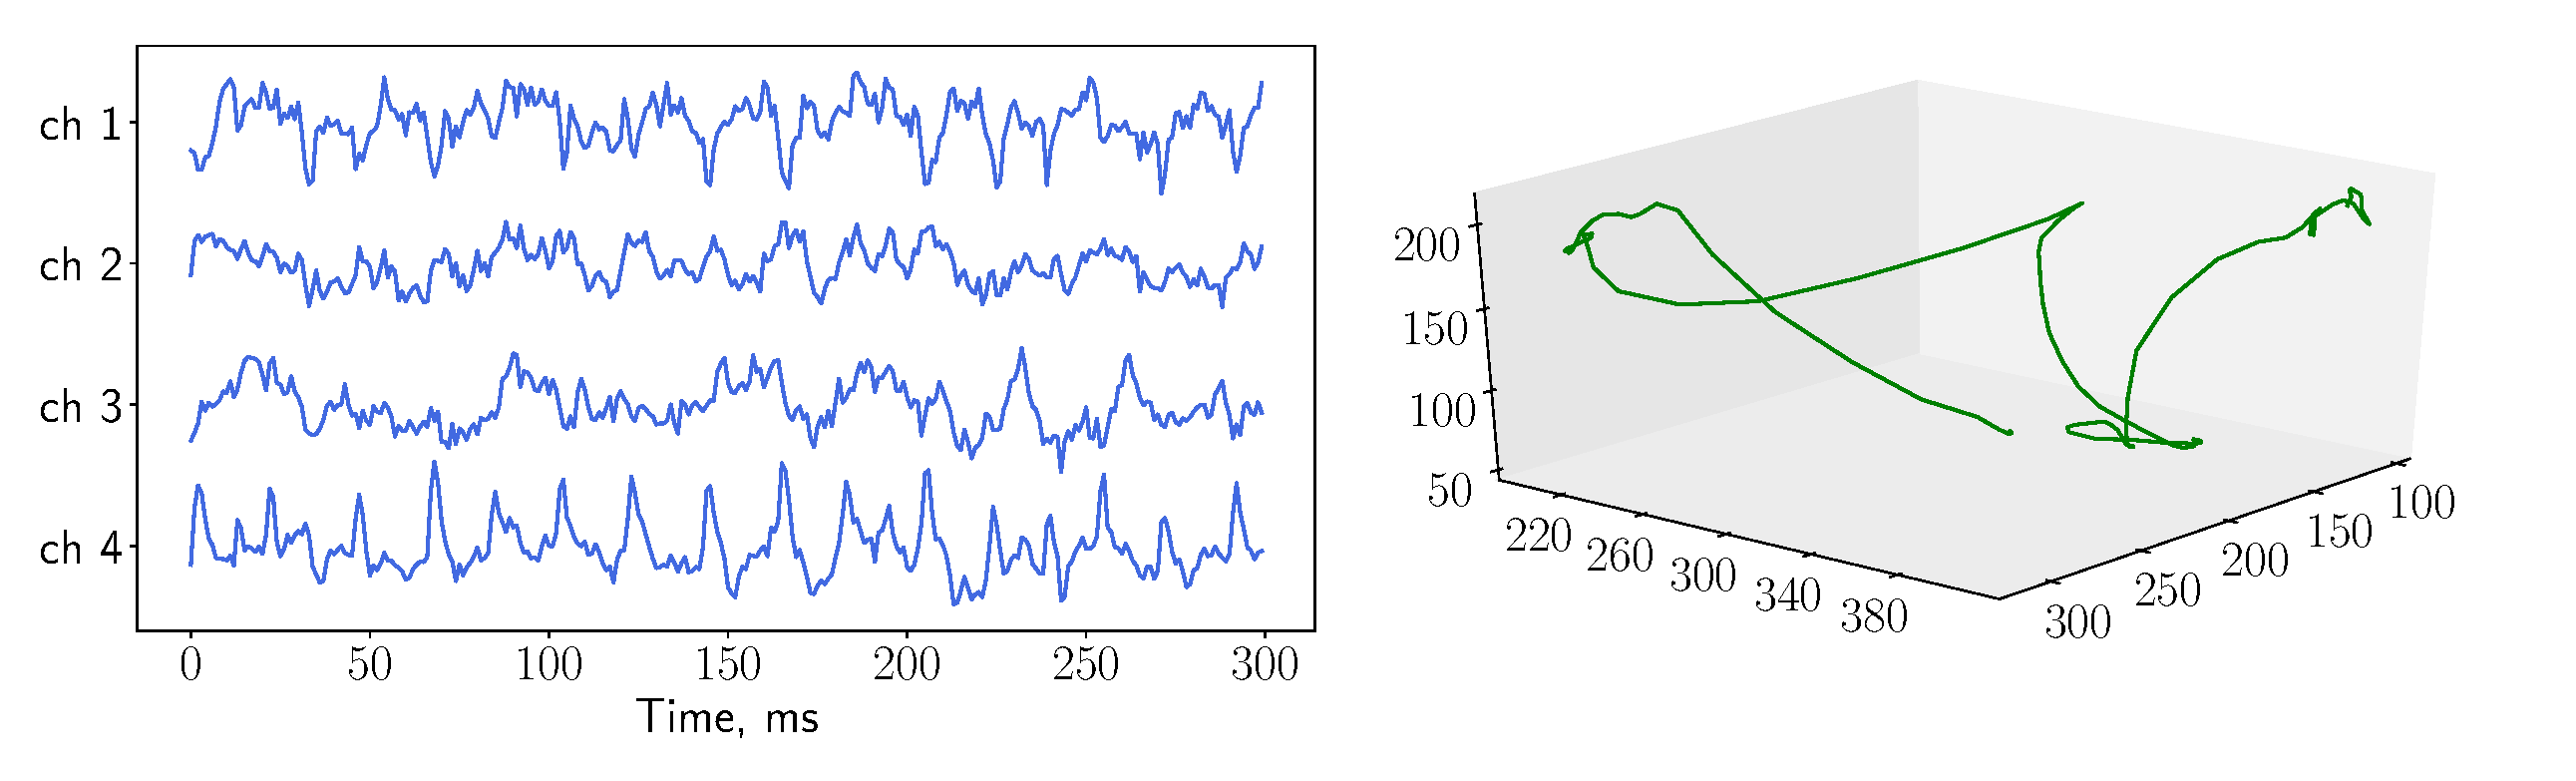
\includegraphics[width=\linewidth]{figs/ecog_data}
	\end{figure}
\end{block}

\[
	\bX \in \bbR^{m \times (32 \cdot 27)}; \quad 
	\bY = 
	\begin{pmatrix}
	x_1 \,\, y_1 \,\, z_1 & \dots & x_{k\hphantom{+1}} \,\, y_{k\hphantom{+1}} \,\, z_{k\hphantom{+1}}\\
	x_2 \,\, y_2 \,\, z_2 & \dots & x_{k + 1} \,\, y_{k + 1} \,\, z_{k + 1}\\
	 \dots & \dots & \dots  \\
	x_m \, y_m \, z_m & \dots & x_{m + k} \, y_{m + k} \, z_{m + k}
	\end{pmatrix} \in \bbR^{m \times 3k}.
\]
\vspace{0.5cm}

\hrulefill \\
\url{http://neurotycho.org}
\end{frame}
%--------------------------------------------------------------------------------
\begin{frame}{Data redundancy}
	\begin{figure}
		\begin{minipage}{.5\linewidth}
			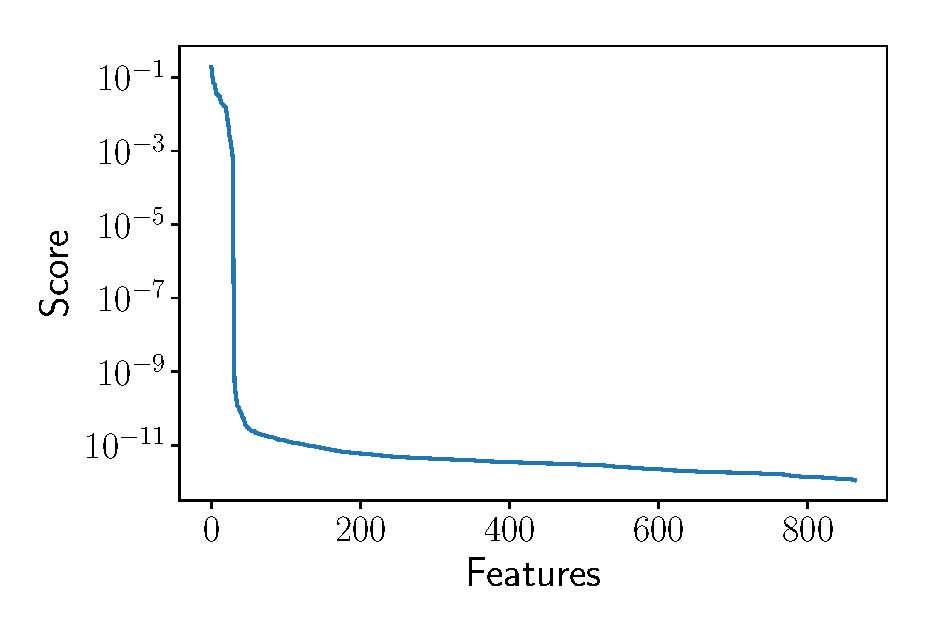
\includegraphics[width=\linewidth]{figs/feature_scores_ex.eps}
		\end{minipage}%
		\begin{minipage}{.5\linewidth}
			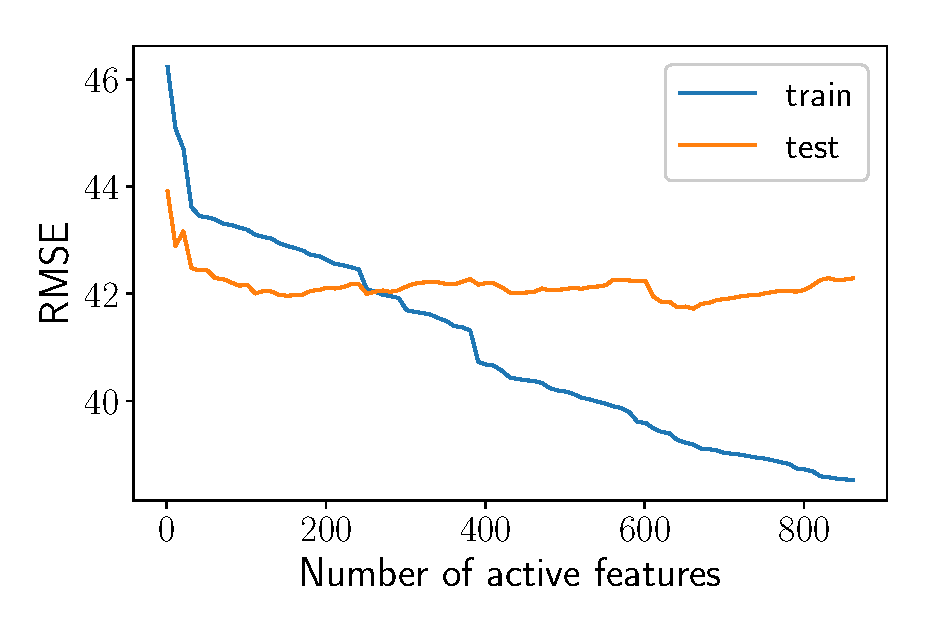
\includegraphics[width=\linewidth]{figs/train_test_qpfs.eps}
		\end{minipage}
		\centering
		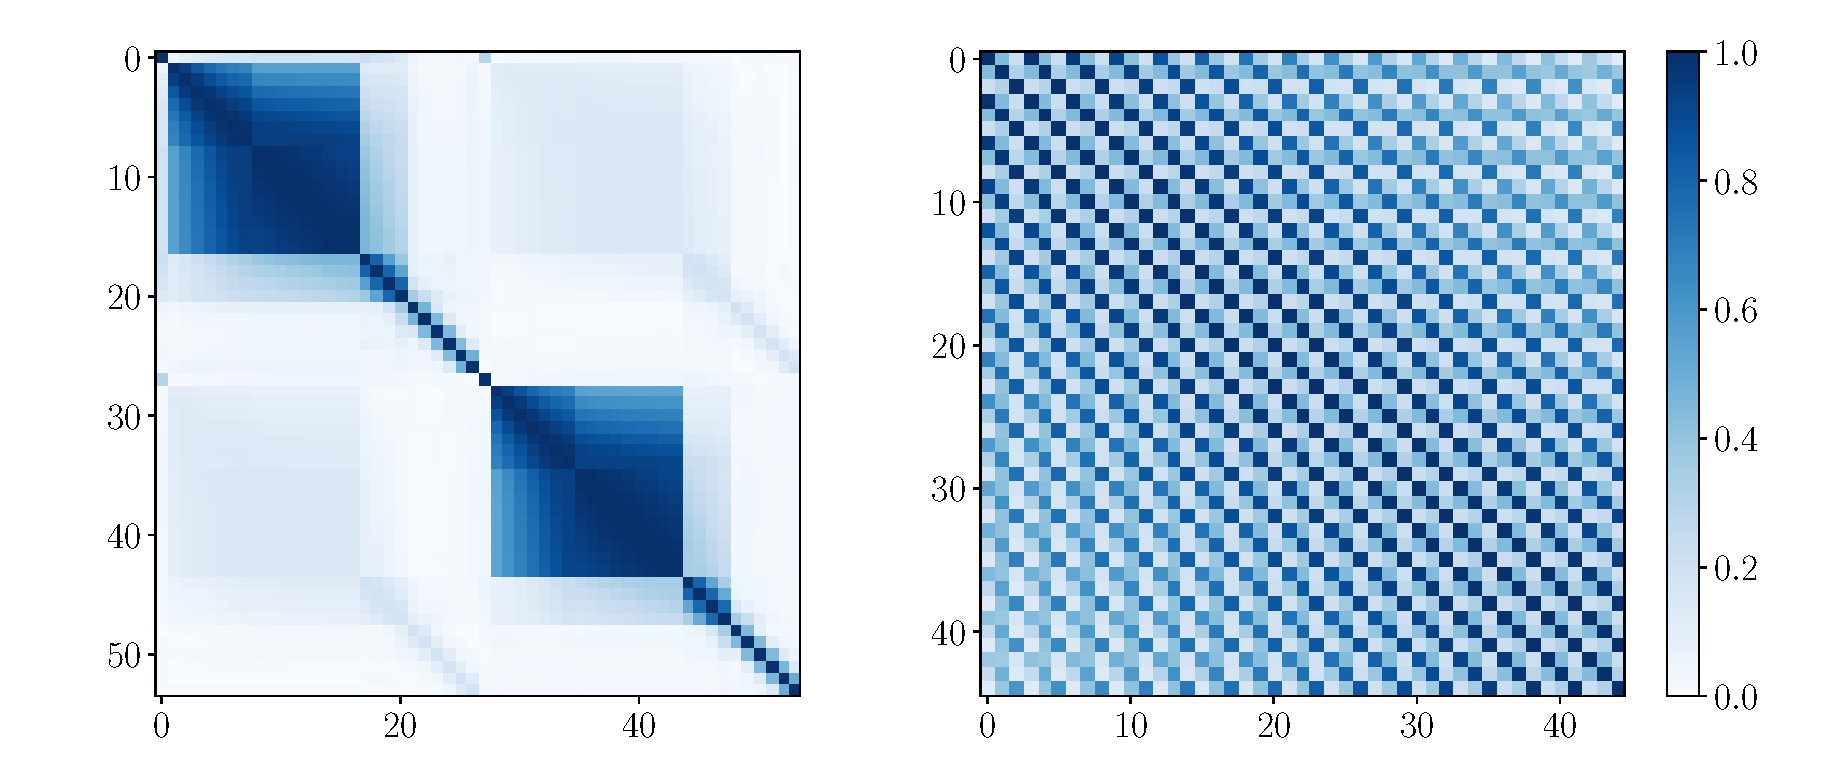
\includegraphics[width=0.9\linewidth]{figs/corr_matrix.eps}
	\end{figure}
\end{frame}
%--------------------------------------------------------------------------------
\begin{frame}{Target importances}
\begin{figure}
	\begin{minipage}{.5\linewidth}
			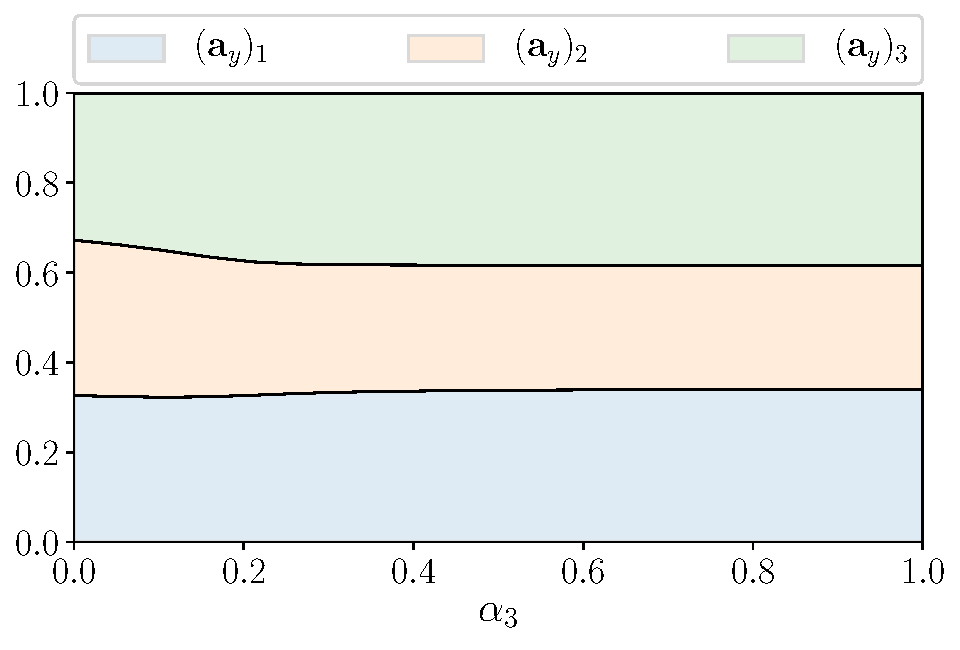
\includegraphics[width=\linewidth]{figs/features_vs_alpha_ecog_3.pdf}
	\end{minipage}%
	\begin{minipage}{.5\linewidth}
			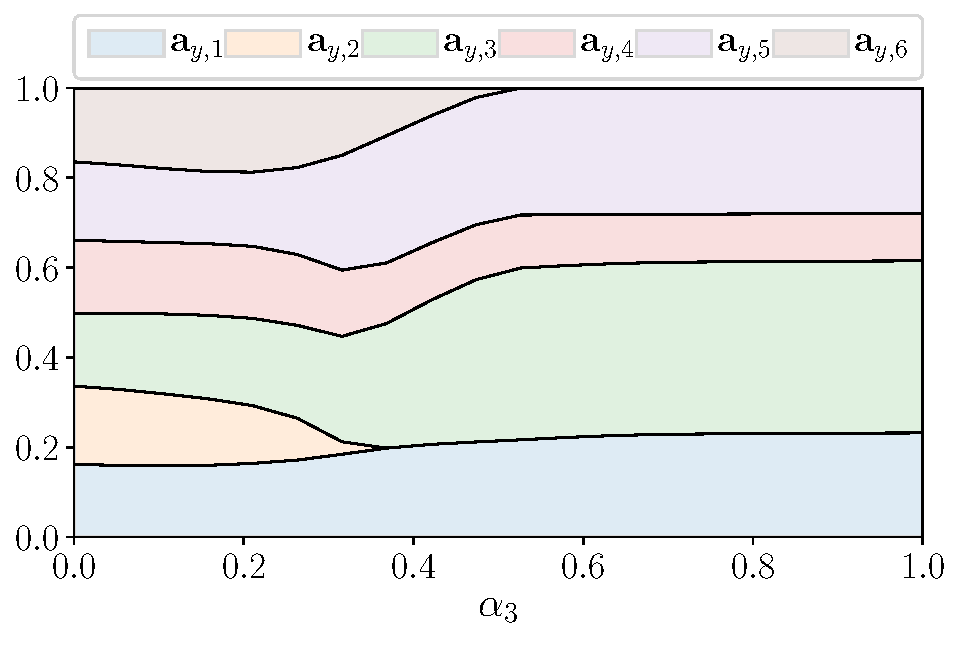
\includegraphics[width=\linewidth]{figs/features_vs_alpha_ecog_6.pdf}
	\end{minipage}\par\medskip
		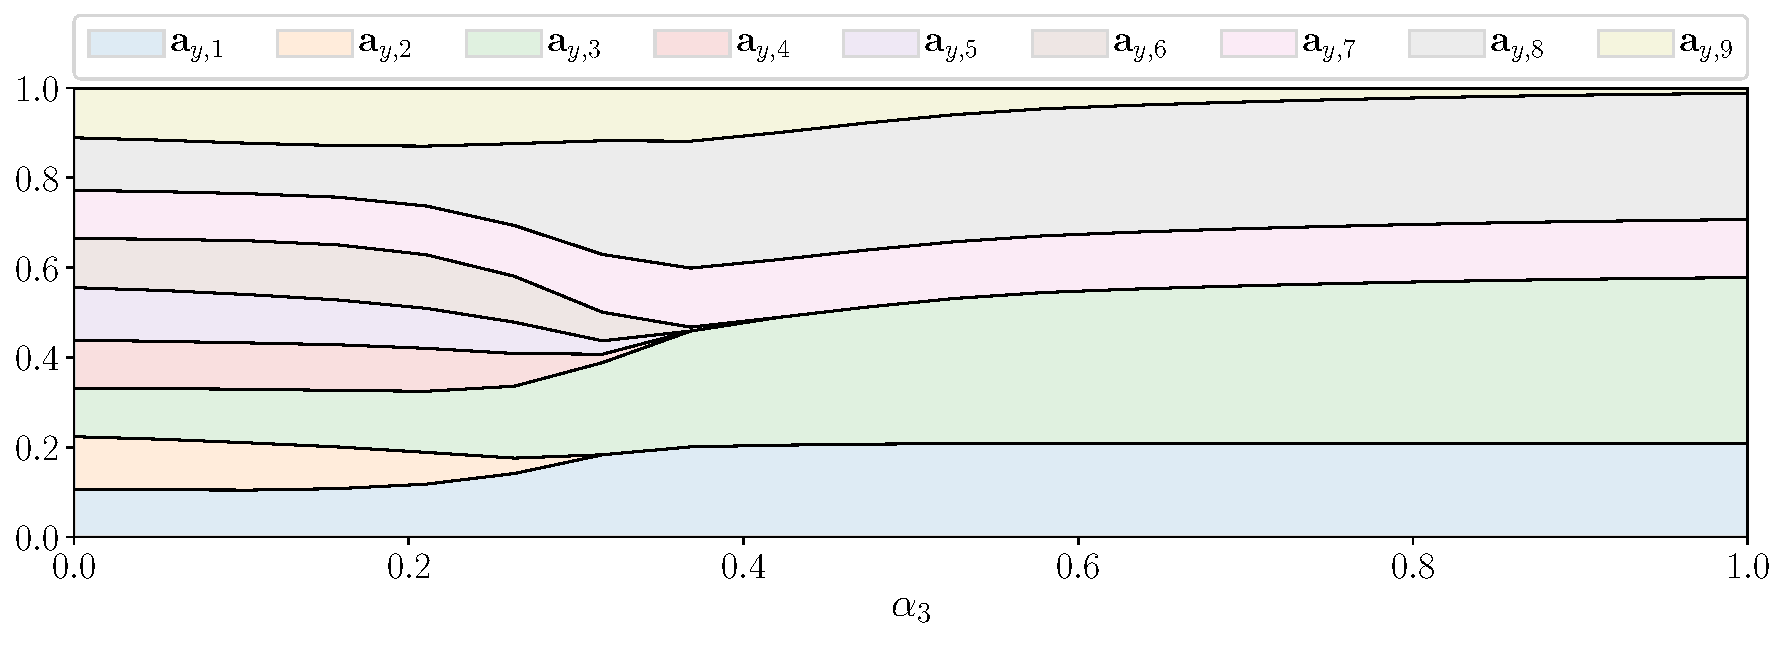
\includegraphics[width=\linewidth]{figs/features_vs_alpha_ecog_9.pdf}
\end{figure}
\end{frame}
%--------------------------------------------------------------------------------
\begin{frame}{Autoregression step = 1}
	\begin{figure}
		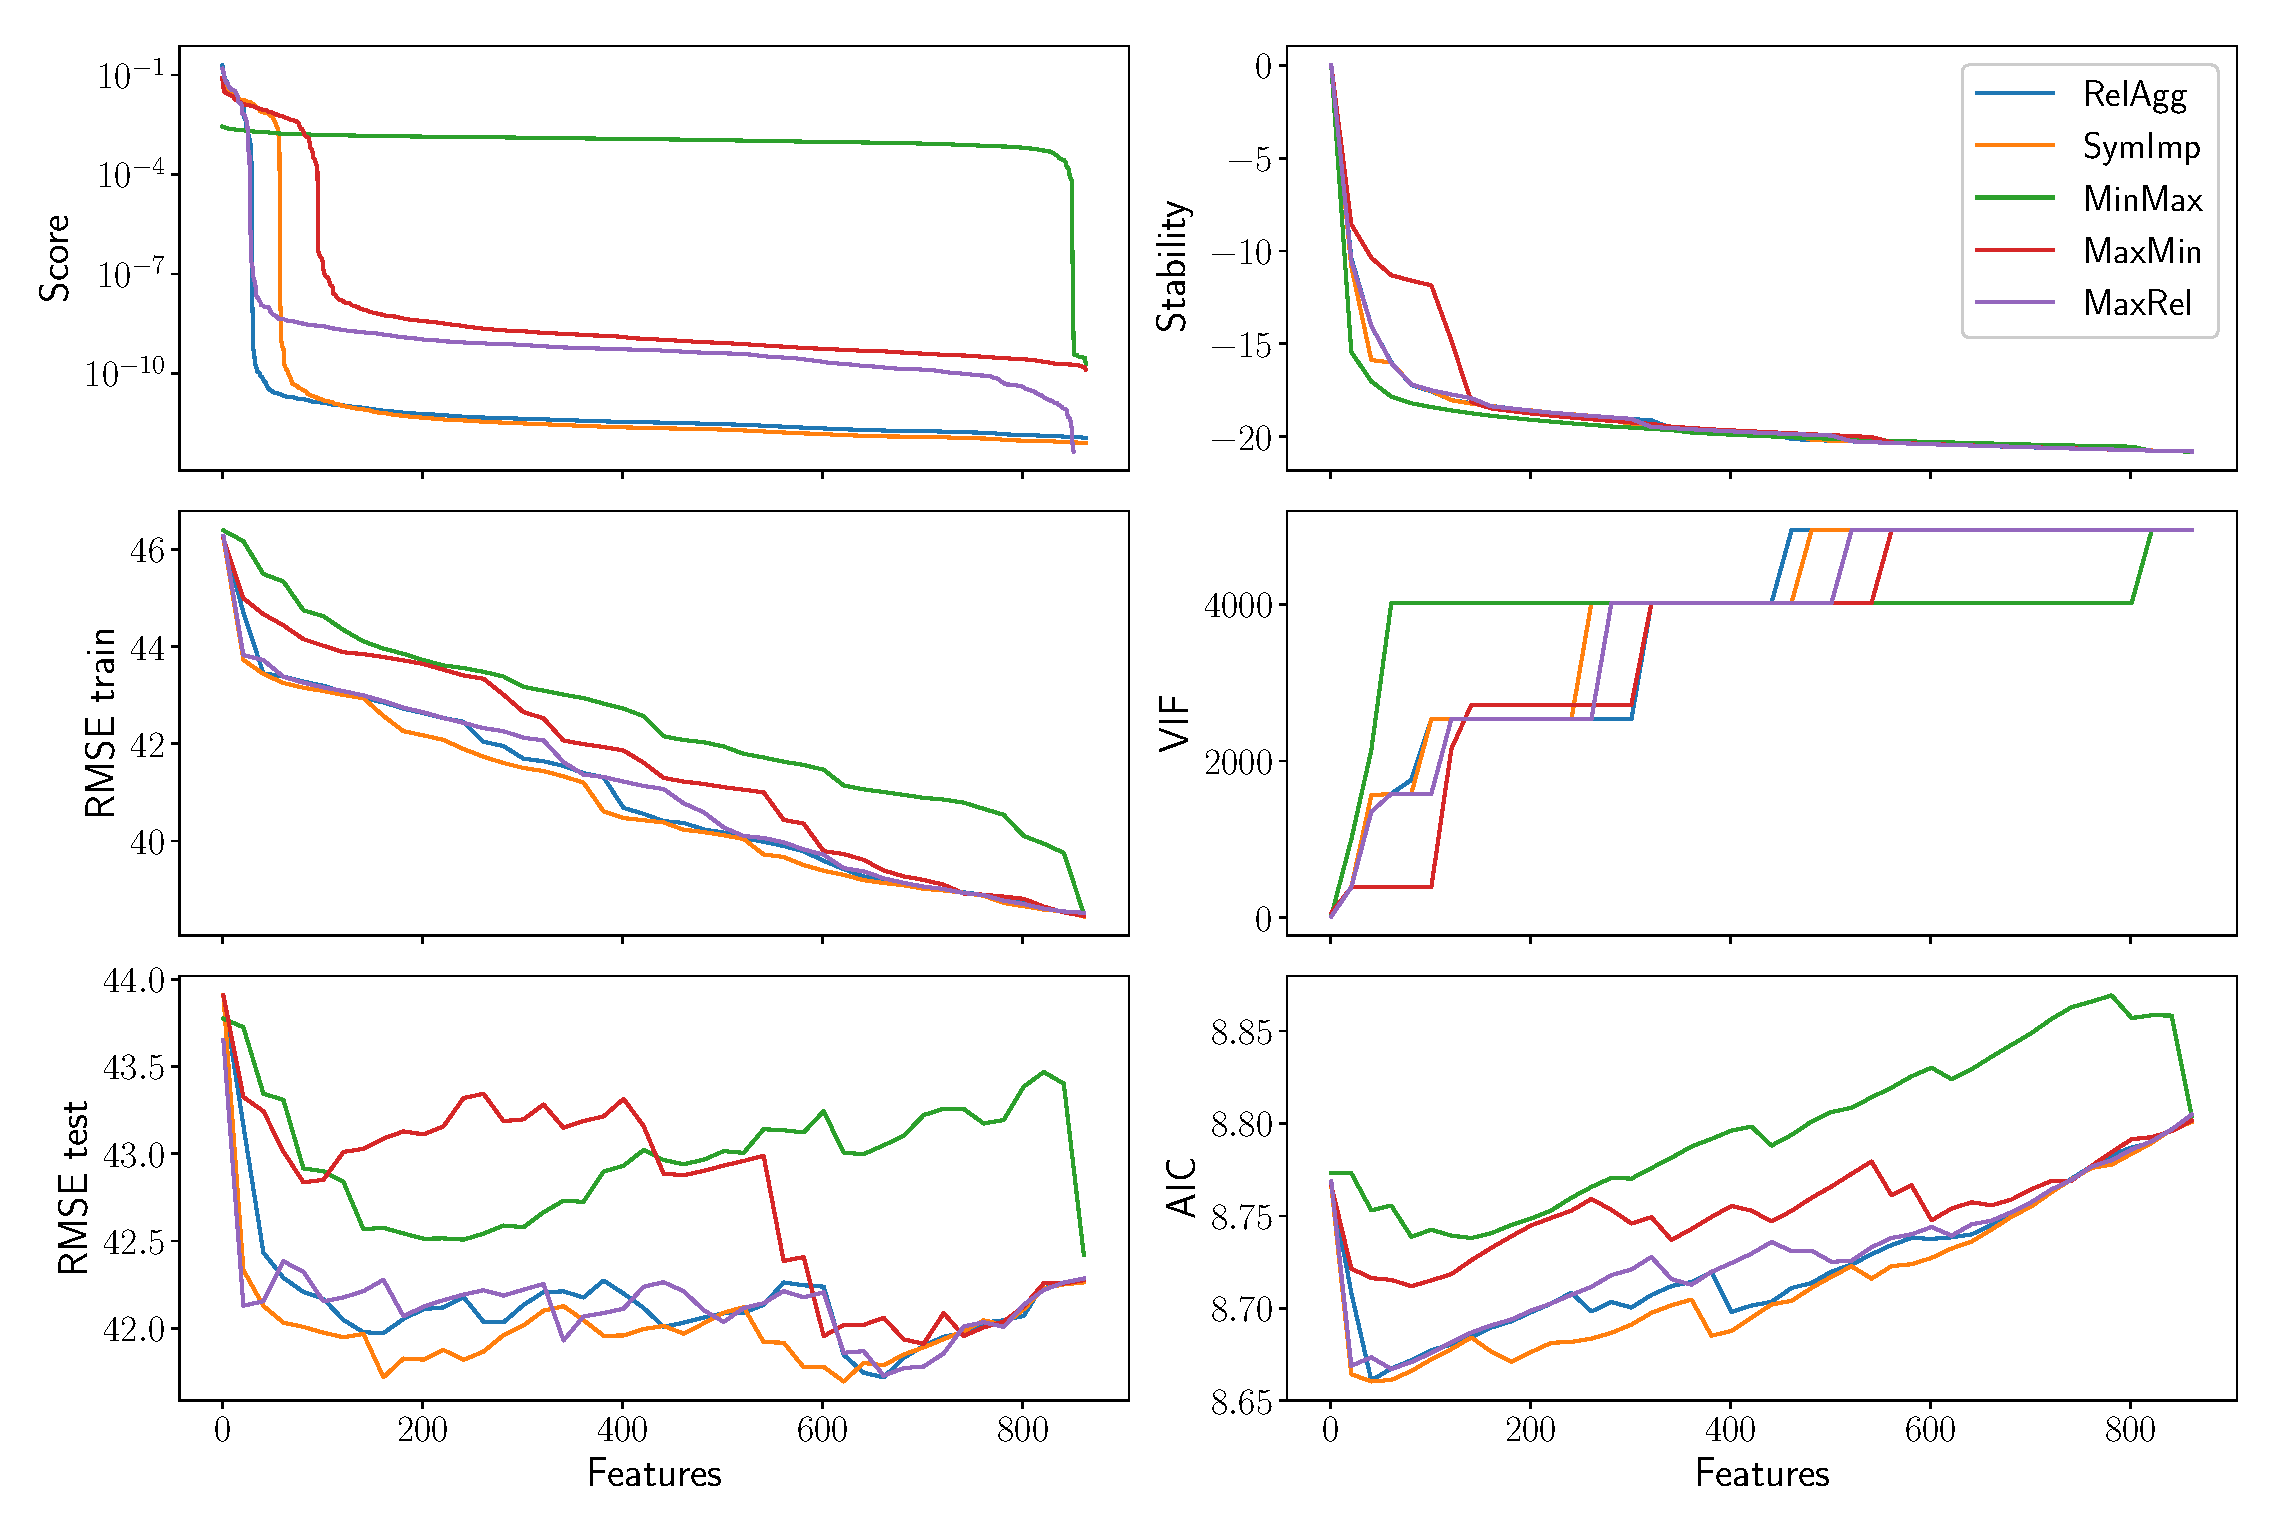
\includegraphics[width=\linewidth]{figs/ecog_3_1_metrics.eps}
	\end{figure}
\end{frame}
%--------------------------------------------------------------------------------
\begin{frame}{Autoregression step = 30}
	\begin{figure}
		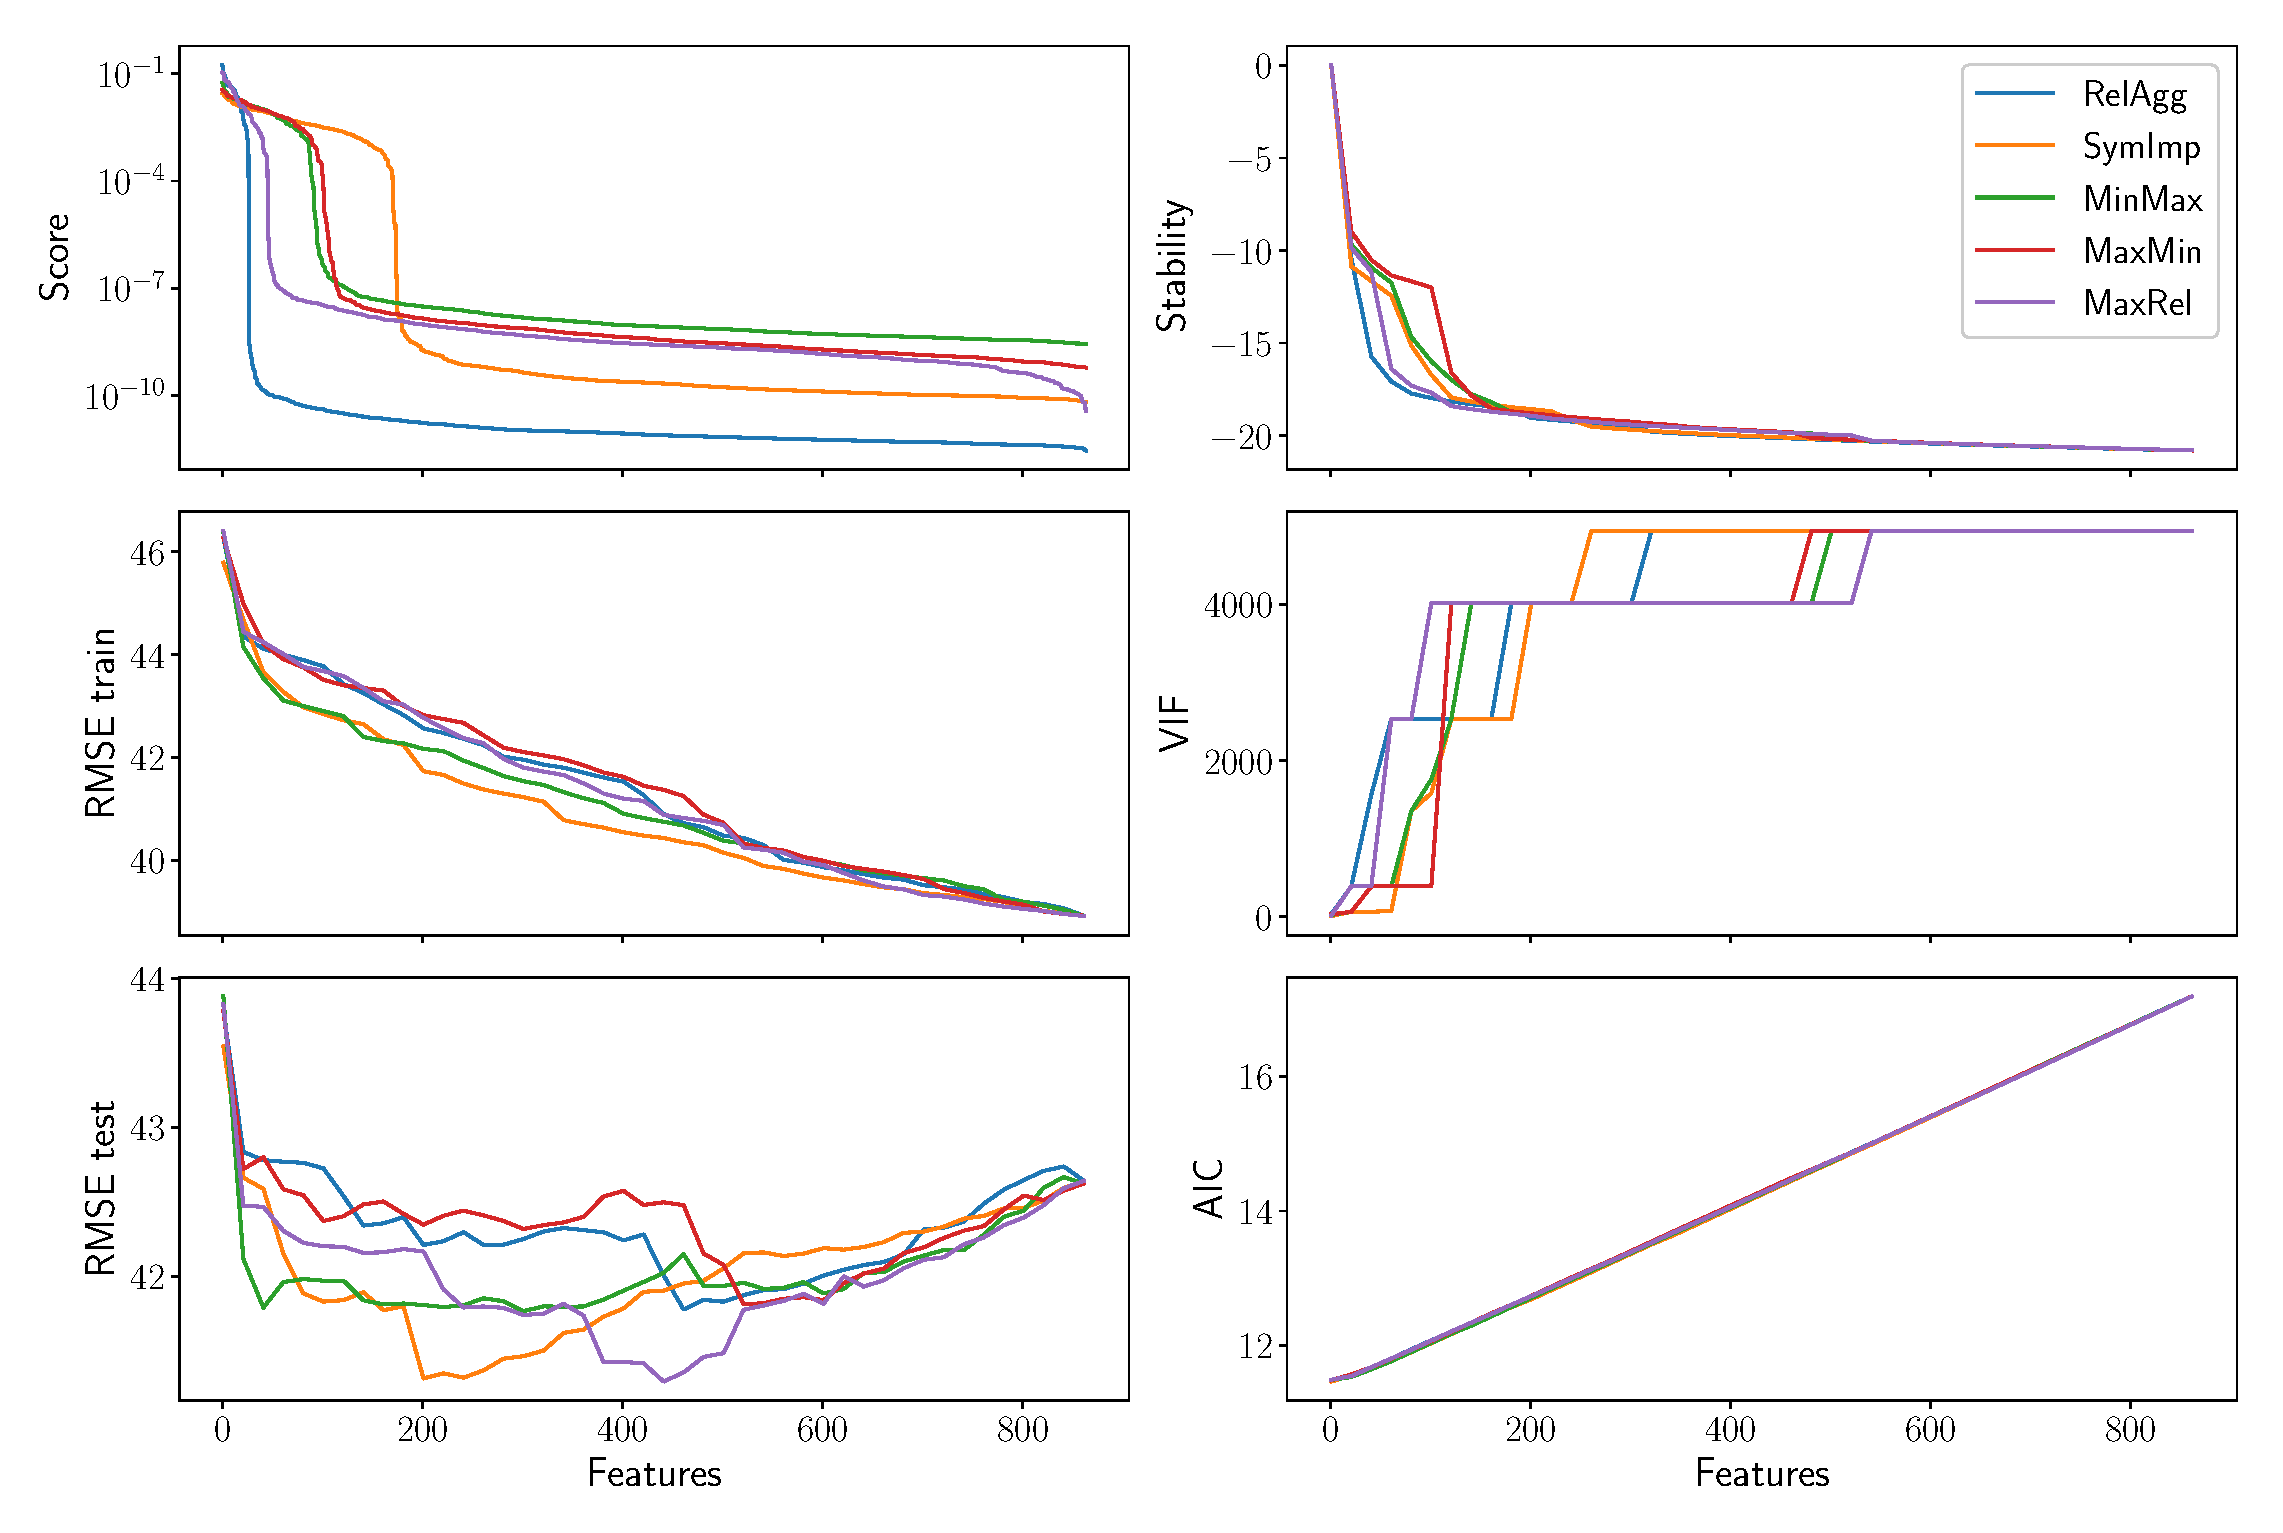
\includegraphics[width=\linewidth]{figs/ecog_3_15_metrics.eps}
	\end{figure}
\end{frame}
%--------------------------------------------------------------------------------
\begin{frame}{Conclusion}
	\begin{itemize}
		\item BCI signal decoding problem is investigated.
		\item Feature selection algorithms for spatio-temporal data are proposed.
		\item Suggested algorithms are explored and compared.
	\end{itemize}
	\begin{block}{Publications}
		\begin{itemize}
			\item Isachenko~R. et al. Feature Generation for Physical Activity Classification. \emph{Artificial Intellegence and decision making}, submitted.
			\item Isachenko~R., Strijov~V. Quadratic programming optimization for Newton method. \emph{Lobachevskii Journal of Mathematics}, submitted.
			\item Isachenko~R., Vladimirova~M., Strijov~V. Dimensionality reduction for time series decoding and forecasting problems. Ready for submission.
		\end{itemize}
	\end{block}
\end{frame}
%--------------------------------------------------------------------------------
\begin{frame}{}
\end{frame}
%--------------------------------------------------------------------------------
\begin{frame}{Feature categorization}
	\begin{enumerate}
		\item non-relevant features
		\[
		\left\{j: \text{corr}(\bchi_j, \bnu_k) = 0, \, \forall k \in \{1, \dots, r\}\right\};
		\]
		\item non-$\bX$-correlated features, which are relevant to non-$\bY$-correlated targets
		\[
		\left\{j: \left(\text{VIF}(\bchi_j) < 10\right) \, \text{and} \, \left(\text{VIF}(\bnu_k) < 10 , \, \forall k \in \{1, \dots, r\}: \,  \text{corr}(\bchi_j, \bnu_k) \neq 0 \right)\right\};
		\]
		\item non-$\bX$-correlated features, which are relevant to $\bY$-correlated targets
		\[
		\left\{j: \left(\text{VIF}(\bchi_j) < 10\right) \, \text{and} \, \left( \exists k \in \{1, \dots, r\}: \text{VIF}(\bnu_k) > 10 \,\, \& \,\, \text{corr}(\bchi_j, \bnu_k) \neq 0 \right)\right\};
		\]
		\item $\bX$-correlated features, which are relevant to non-$\bY$-correlated targets
		\[
		\left\{j: \left(\text{VIF}(\bchi_j) > 10\right) \, \text{and} \, \left(\text{VIF}(\bnu_k) < 10 , \, \forall k \in \{1, \dots, r\}: \,  \text{corr}(\bchi_j, \bnu_k) \neq 0 \right)\right\};
		\]
		\item $\bX$-correlated features, which are relevant to $\bY$-correlated targets
		\[
		\left\{j: \left(\text{VIF}(\bchi_j) > 10\right) \, \text{and} \, \left( \exists k \in \{1, \dots, r\}: \text{VIF}(\bnu_k) > 10 \,\, \& \,\, \text{corr}(\bchi_j, \bnu_k) \neq 0 \right)\right\}.
		\]
	\end{enumerate}
	
	\[
	r = \text{corr} (\bchi, \bnu), \quad t = \frac{r \sqrt{m - 2}}{1 - r^2} \sim \text{St} (m - 2).
	\]
	\[
	\text{VIF}(\bchi_j) = \frac{1}{1 - R_j^2}, \quad \text{VIF}(\bnu_k) = \frac{1}{1 - R_k^2},
	\]
	where $R_j^2$($R_k^2$) are coefficients of determination for the regression of $\bchi_j$($\bnu_k$) on the other features(targets).
\end{frame}
%--------------------------------------------------------------------------------
\begin{frame}{Problem Statement}
\begin{minipage}{0.6\linewidth}
	\begin{figure}
		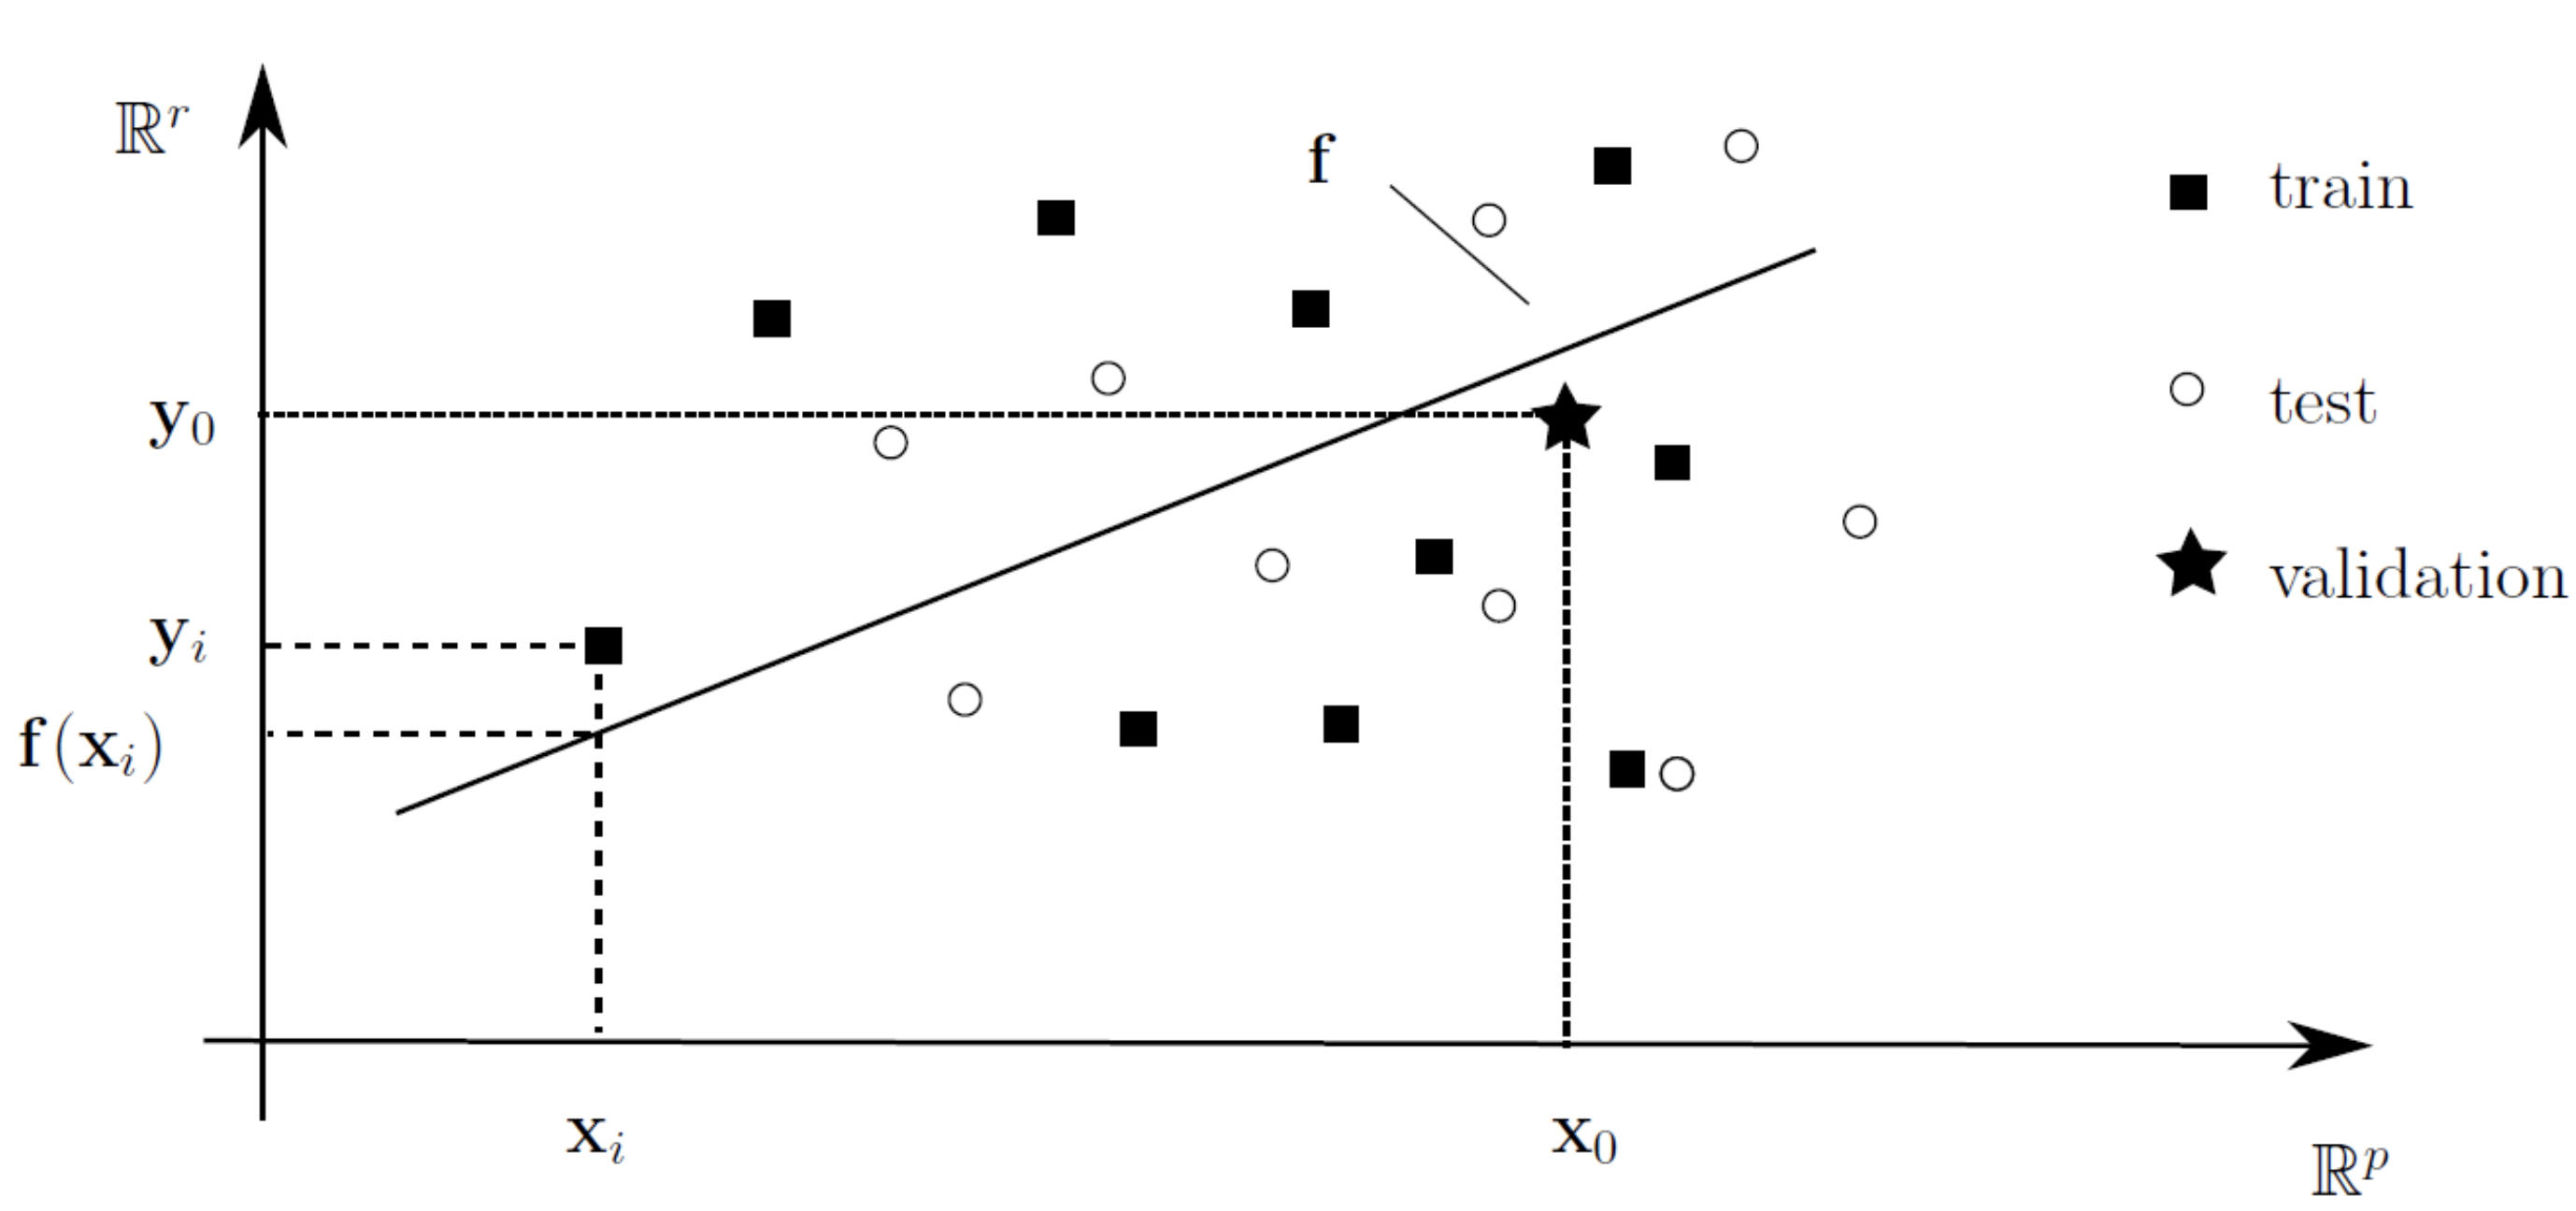
\includegraphics[width=1.1\linewidth]{figs/forecast_scheme}
	\end{figure}
	\begin{block}{Partial Least Squares (PLS)}
	\vspace{-0.5cm}
	\begin{align*}
		\underset{m \times n}{\vphantom{\bQ}\bX} 
		&= \underset{m \times l}{\vphantom{\bQ}\bT} \cdot \underset{l \times n}{\vphantom{\bQ}\bP^{T}} + \underset{m \times n}{\vphantom{\bQ}\bF} 
		= \sum_{k=1}^l \underset{m \times 1}{\vphantom{\bp_k^{T}}\bt_k} \cdot \underset{1 \times n}{\bp_k^{T}} + \underset{m \times n}{\vphantom{\bp_k^{T}}\bF}\\
		\underset{m \times r}{\vphantom{\bQ}\bY} 
		&= \underset{m \times l}{\vphantom{\bQ}\bU} \cdot \underset{l \times r}{\bQ^{T}} + \underset{m \times r}{\vphantom{\bQ}\bE}
		=  \sum_{k=1}^l  \underset{m \times 1}{\vphantom{\bq_k^{T}}\bt_k} \cdot \underset{1 \times r}{\bq_k^{T}} +  \underset{m \times r}{\vphantom{\bq_k^{T}}\bE}
	\end{align*}
	\end{block}
	\begin{equation*}
		\mathbf{\hat{Y}} = \mathbf{T}\text{diag}(\boldsymbol{\beta}) \bQ^{T} = \bX \bTheta.
	\end{equation*}
\end{minipage}%
\begin{minipage}{0.4\linewidth}
	
	\begin{figure}
		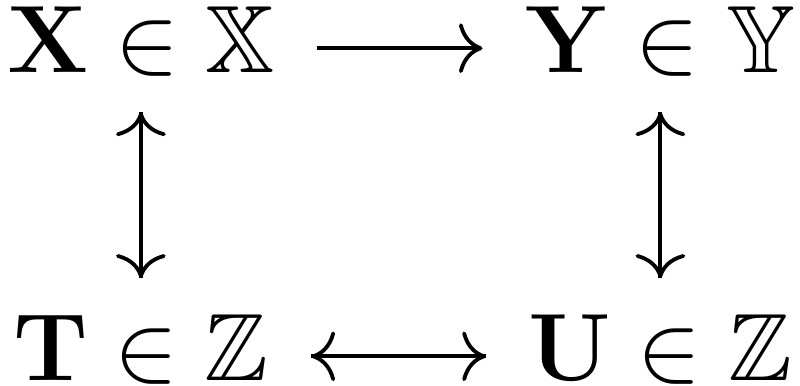
\includegraphics[width=0.6\linewidth]{figs/diagram}
	\end{figure}
	\vspace{1cm}
	\begin{itemize}
		\item map $\bX$ into low-dimensional~$\bT$;
		\item map $\bY$ into low-dimensional~$\bU$;
		\item maximize correlation between $\bt_k$ and $\bu_k$.
	\end{itemize}
\end{minipage}
\end{frame}
%--------------------------------------------------------------------------------
\begin{frame}{PLS Example}
	\begin{figure}
		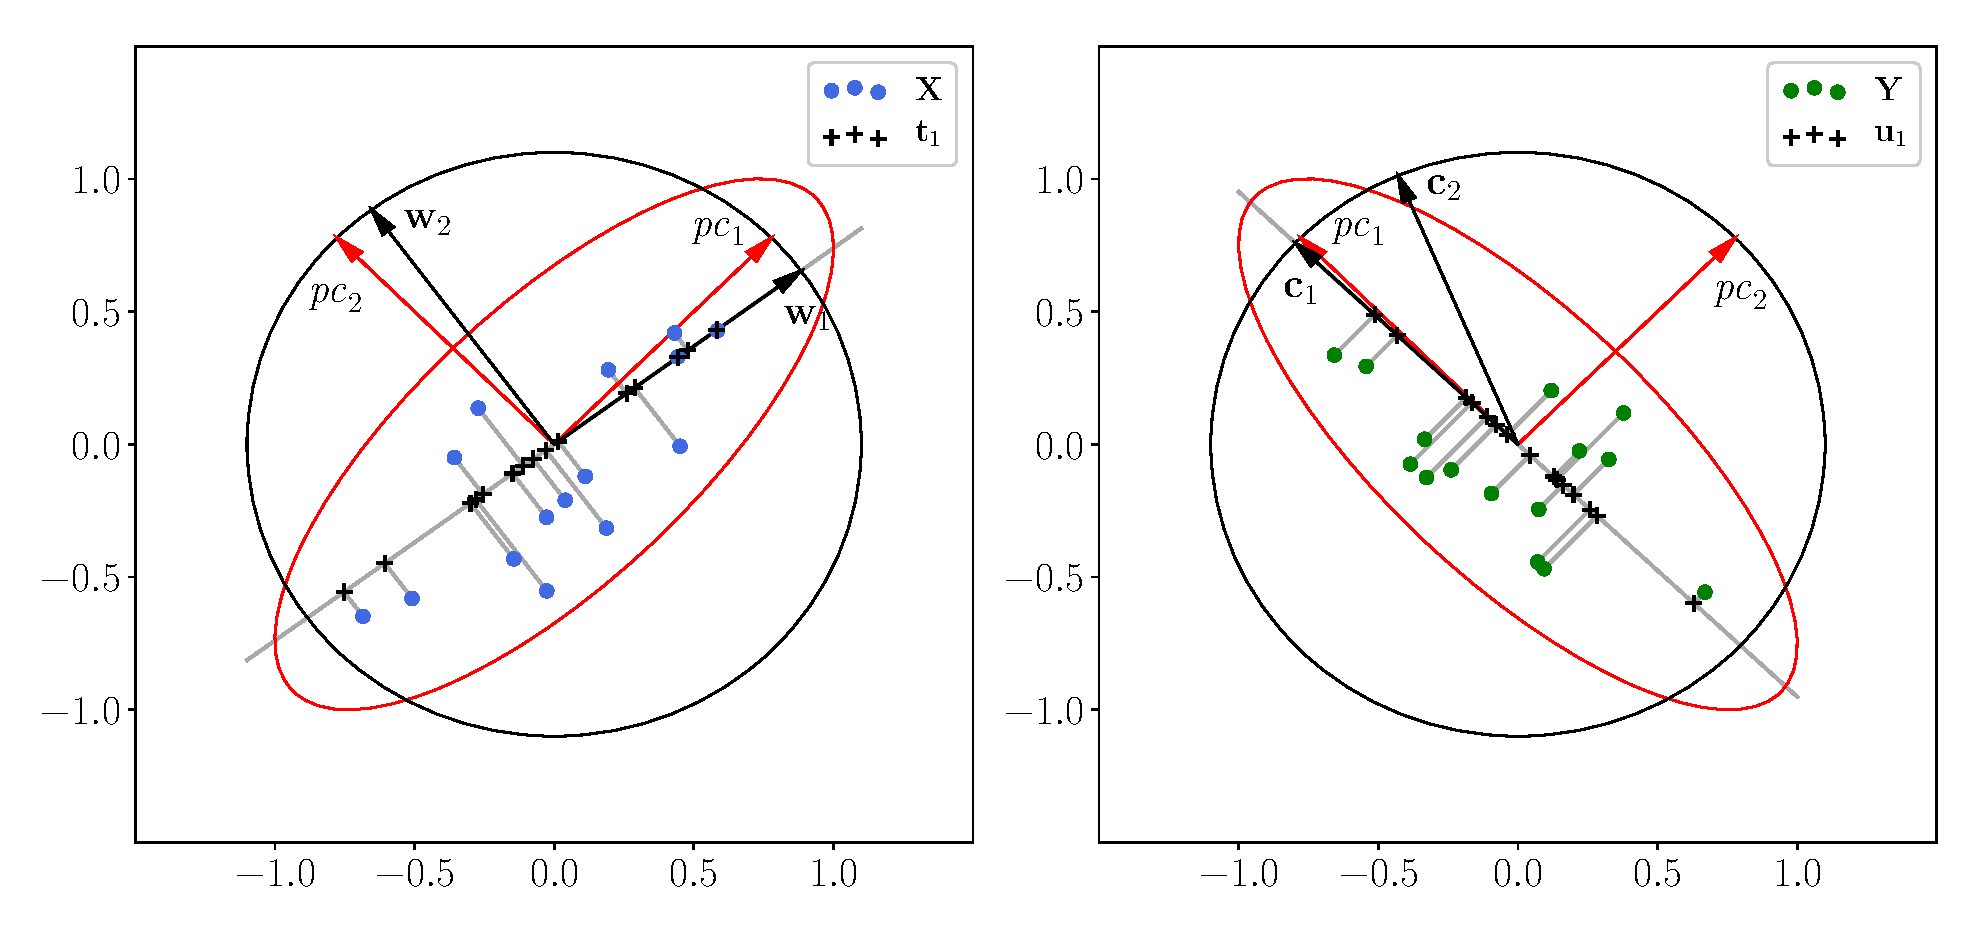
\includegraphics[width=\linewidth]{figs/PLSFigure.eps}
		\caption{The result of the PLS algorithm for the case $n = r = l = 2$.}
	\end{figure}
\end{frame}
%--------------------------------------------------------------------------------
\begin{frame}{Computational experiment}
	\begin{minipage}{0.55\textwidth}
		\begin{block}{Datasets}
			\vspace{0.35cm}
			\begin{itemize}
				\item energy consumption
				\item electrocorticogram signals (ECoG)
			\end{itemize}
		\end{block}
		\vspace{0.5cm}
	\end{minipage}%
	\begin{minipage}{0.45\textwidth}
		\begin{block}{Autoregressive approach}
				\[
				\mathbf{X} = 
				\begin{pmatrix}
				x_1 & x_2 & \dots & x_n \\
				x_2 & x_3 & \dots & x_{n+1} \\
				\dots & \dots & \dots & \dots \\
				x_{T-n+1} & x_{T-n+2} & \dots & x_T
				\end{pmatrix}
				\]
		\end{block}
	\end{minipage}
	\begin{block}{ECoG data}
	\begin{figure}
		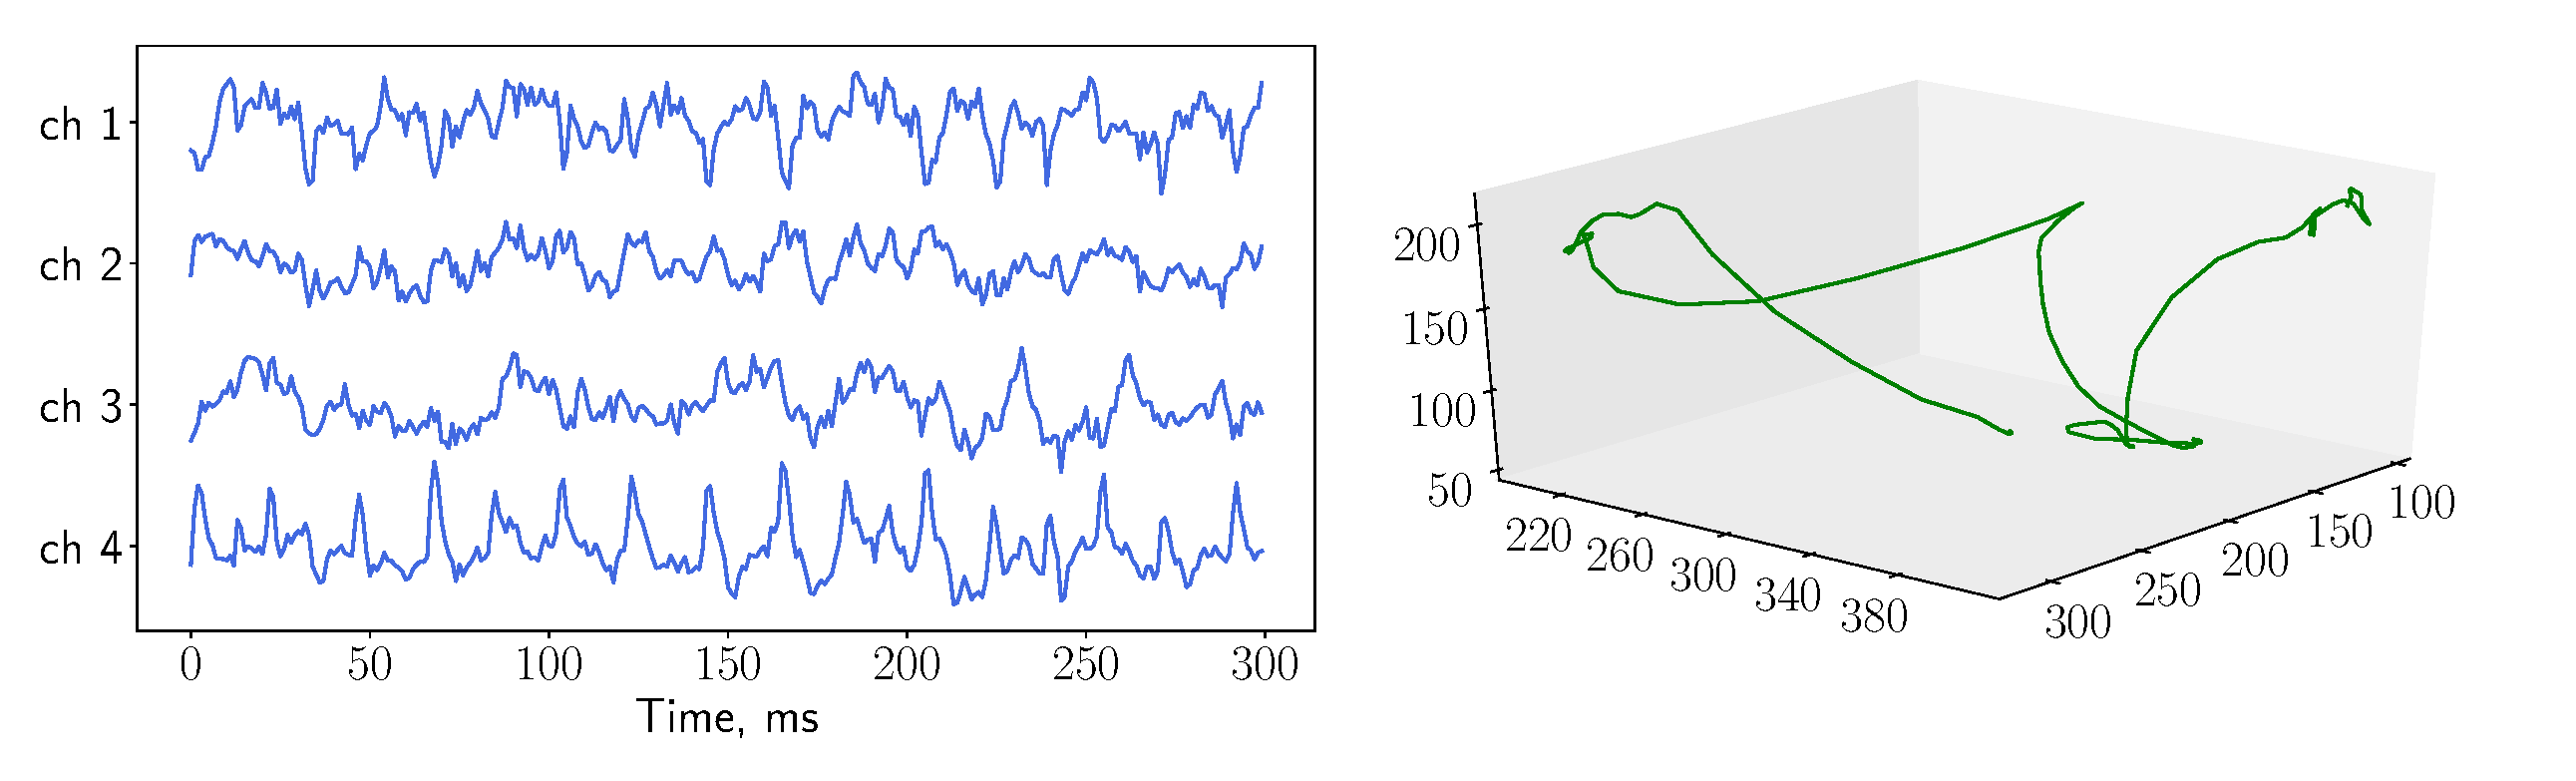
\includegraphics[width=\linewidth]{figs/ecog_data}
	\end{figure}
	\end{block}
\end{frame}
%--------------------------------------------------------------------------------
\begin{frame}{Computational experiment}
	\begin{block}{Energy consumption}
	\begin{figure}
		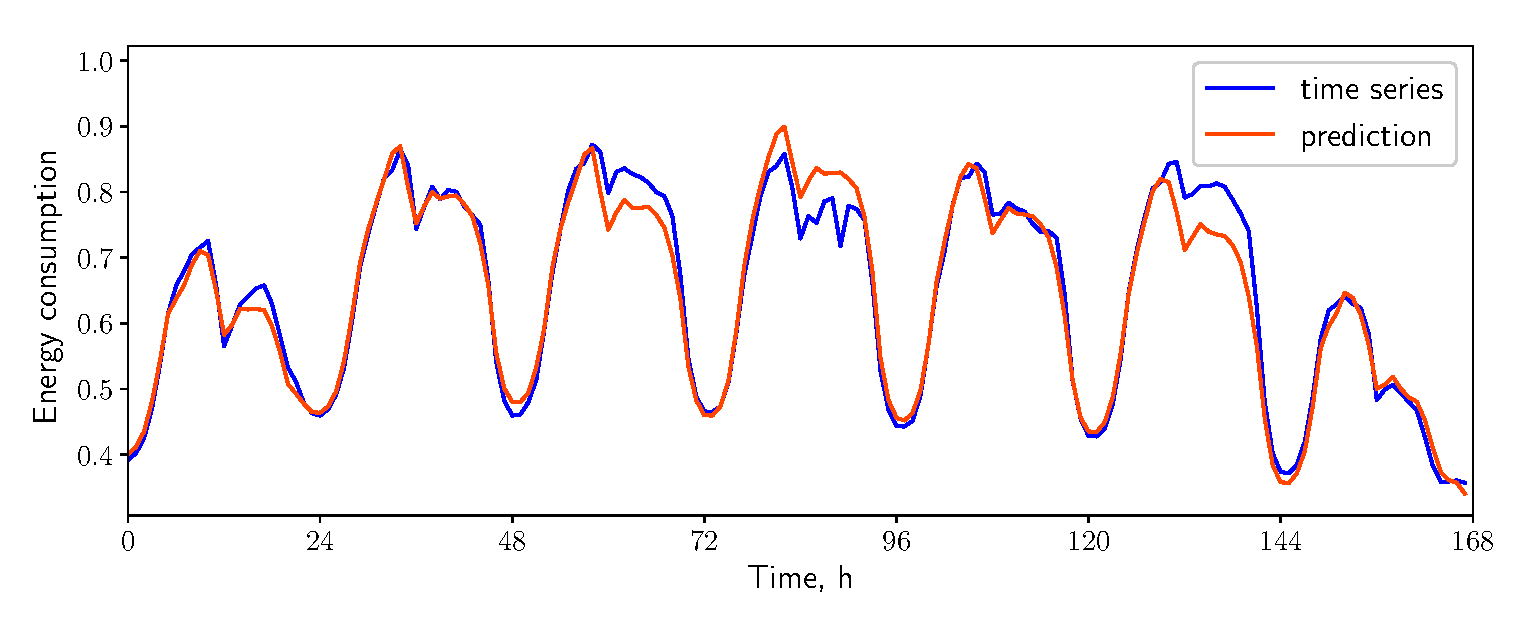
\includegraphics[width=0.8\linewidth]{figs/energy_prediction_pres.eps}
	\end{figure}
	\vspace{-0.5cm}
	\end{block}
	\begin{block}{Results}
	\begin{itemize}
		\item Space dimensionalities: $\bX = 700 \times (24 \cdot 7)$ , $\bY = 700 \times 24$.
		\item Dimensionality of latent space: 14
		\item NMSE: 0.047
	\end{itemize}
	\end{block}
\end{frame}
%--------------------------------------------------------------------------------
\begin{frame}{Computational experiment}
	\begin{block}{ECoG}
	\begin{figure}
		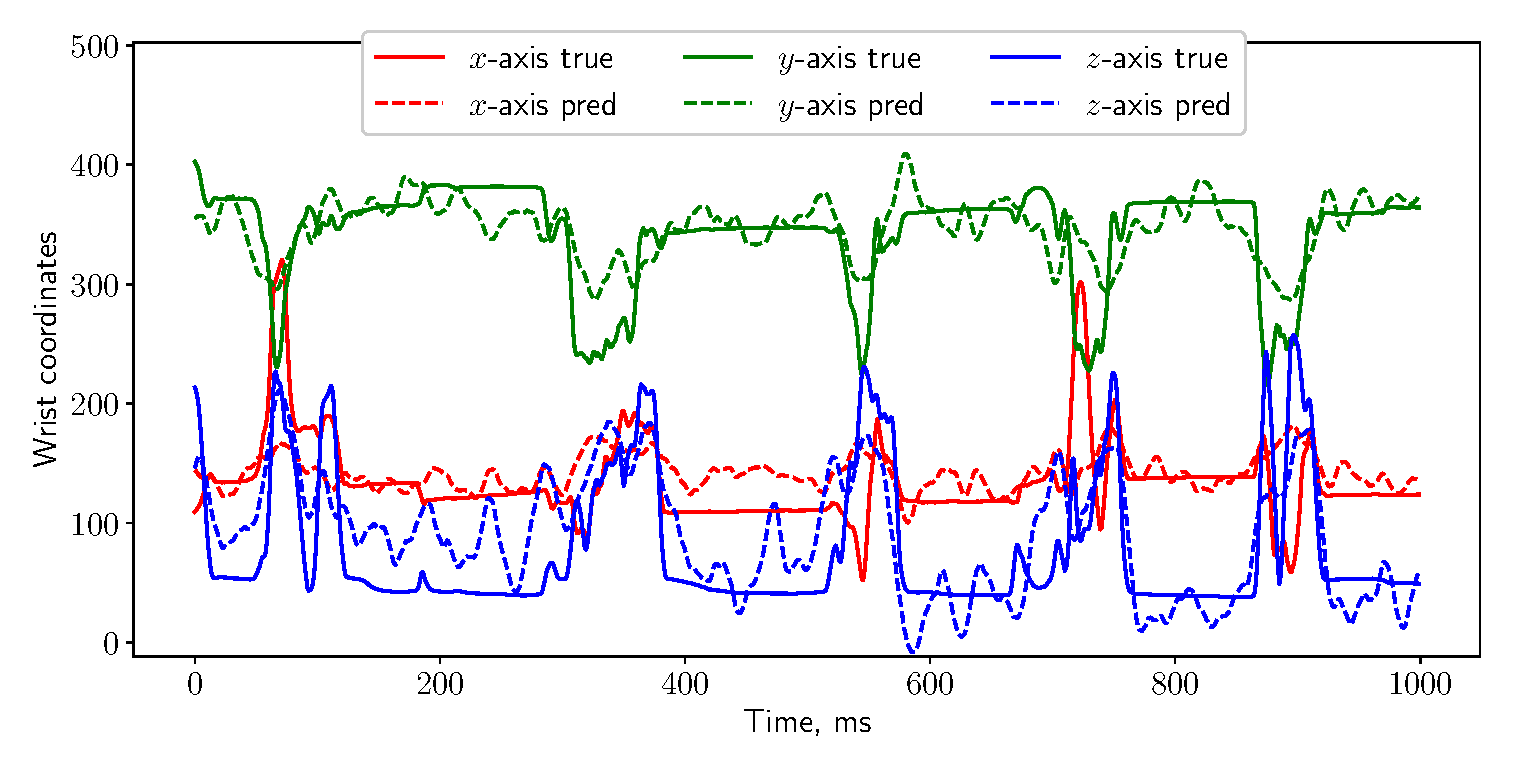
\includegraphics[width=0.8\linewidth]{figs/ecog_prediction_pres.eps}
	\end{figure}
	\end{block}
	\begin{block}{Results}
		\begin{itemize}
			\item Space dimensionalities: $\bX = 13000 \times (864 \cdot 18)$ , $\bY = 13000 \times 3$.
			\item Dimensionality of latent space: 16
			\item NMSE: 0.731
		\end{itemize}
	\end{block}
\end{frame}
%--------------------------------------------------------------------------------
\begin{frame}{Quadratic Programming Model Selection}
	\begin{block}{QPFS}
		\begin{itemize}
			\item works for linear problems;
			\item does not take into account the model;
			\item ignores the structure of the target space.
		\end{itemize}
	\end{block}
	\begin{block}{Problem}
		\begin{equation*}
			\underbrace{(1 - \alpha) \bz^{T} \bQ \bz}_{\text{Sim}} - \underbrace{\vphantom{()}\alpha \mathbf{b}^{T} \bz}_{\text{Rel}} \rightarrow \min_{\substack{\bz \in \bbR^p_+ \\ \|\bz\|_1 = 1}}.
		\end{equation*}
	\end{block}
	\begin{itemize}
		\item $\bz \in \bbR^p$ --- weight importances;
		\item $\bQ \in \bbR^{p \times p}$ - pairwise weights interactions;
		\item $\mathbf{b} \in \bbR^p$ - weight relevances to the target vector.
	\end{itemize}
	\begin{equation*}
		w_j = 0 \Leftrightarrow z_j < \tau.
	\end{equation*}
\end{frame}
\end{document} 
